\documentclass[a4paper]{report}
\usepackage[utf8]{inputenc}
\usepackage[T1]{fontenc}
\usepackage[italian]{babel}
\usepackage{setspace}
\usepackage[left=3cm, right=3cm, top=3cm, bottom=3cm]{geometry}
\usepackage{graphicx}
\usepackage[usenames]{color}
\usepackage{xcolor}
\usepackage{xurl}
\usepackage{hyperref}
\usepackage{array}
\usepackage{caption}
\usepackage{float}
\usepackage{fancyhdr}
\usepackage{datatool}
\usepackage{acronym}
\usepackage[acronym]{glossaries}
\usepackage{textcomp}
\usepackage{csquotes}
\usepackage{tabularx}
\usepackage{makecell}
\usepackage{multirow}
\usepackage{longtable}

% \newcommand{\mintedoptions}{cachedir=/tmp/mint,outputdir=/aux}

\usepackage[outputdir=aux]{minted}

\usepackage[citestyle=authortitle-ibid, backend=biber, hyperref=true]{biblatex}

\definecolor{unipdred}{RGB}{149, 0, 19}
\definecolor{pastelblue}{RGB}{17,93,118}

\hypersetup{
  colorlinks = true,
  linkcolor = black,
  urlcolor = pastelblue,
  breaklinks = true
}
\addbibresource{tesi.bib}
\makeglossaries

\newglossaryentry{g_eai}
{
    name=\textit{Enterprise Application Integration},
    description={\hfill \\
    Il termine si riferisce al processo d'integrazione tra diversi tipi di sistemi informatici di un'azienda attraverso l'utilizzo di software e soluzioni architetturali.
    \hfill \\
    {\footnotesize{\textit{Fonte:} \url{https://it.wikipedia.org/wiki/Enterprise_Application_Integration}}}
    }
}
\newglossaryentry{g_soa}
{
    name=\textit{Service Oriented Architecture},
    description={\hfill \\
    La Service Oriented Architecture definisce un modo per rendere i componenti software riutilizzabili tramite interfacce di servizio. Queste interfacce utilizzano standard di comunicazione comuni in modo da poter essere rapidamente integrate in nuove applicazioni senza dover eseguire ogni volta una profonda integrazione.\\
    Ogni servizio in una SOA incorpora il codice e le integrazioni dei dati necessari per eseguire una funzione aziendale completa e discreta (ad esempio, il controllo del credito del cliente, il calcolo di un pagamento di un prestito mensile o l'elaborazione di un'applicazione ipotecaria). Le interfacce di servizio forniscono un accoppiamento libero, il che significa che possono essere richiamate con poca o nessuna conoscenza della sottostante modalità di implementazione dell'integrazione.\\
    I servizi sono esposti utilizzando protocolli di rete standard - come SOAP (simple object access protocol)/HTTP o JSON/HTTP - per inviare richieste di lettura o modifica dei dati. I servizi sono pubblicati per consentire agli sviluppatori di trovarli rapidamente e riutilizzarli per assemblare nuove applicazioni.
    \hfill \\
    {\footnotesize\textit{Fonte:} \url{https://www.ibm.com/it-it/cloud/learn/soa}}
    }
}

% middleware
% architetture a messaggio
% Integrazione
% Networking
% distribuite? sistemi distribuiti? architetture distribuite? monolitiche?
% big data?
% object Oriented
% design Pattern
% uml?
% Agile (+ manifesto?)
% virtual machine
% container
% event streaming
% request response
% microservizi
% open source
% rest
% proxy?
% asincrono / sincrono
% callback

\newacronym{ict}{ICT}{Information and Communication Technologies}
\newacronym{j2ee}{J2EE}{Java 2 Platform Enterprise Edition}
\newacronym{ejb}{EJB}{Enterprise Java Bean}
\newacronym{cobra}{COBRA}{Common Object Request Broker Architecture}
\newacronym{mom}{MOM}{Message Oriented Middleware}
\newacronym{jms}{JMS}{Java Message Service}
\newacronym{eai}{EAI}{\gls{g_eai}}
\newacronym{oo}{O-O}{Object Oriented}
\newacronym{uml}{UML}{Unified Modeling Language}
\newacronym{cli}{CLI}{Command Line Interface}
\newacronym{soa}{SOA}{\gls{g_soa}}
\newacronym{soap}{SOAP}{Simple Object Access Protocol}
\newacronym{wsdl}{WSDL}{Web Service Description Language}
\newacronym{xml}{XML}{eXtensible Markup Language}
\newacronym{xsd}{XSD}{XML Schema Definition}
\newacronym{json}{JSON}{JavaScript Object Notation}
\newacronym{ws}{WS}{Web Service}
\newacronym{rest}{REST}{REpresentational State Transfer}
\newacronym{sso}{SSO}{Single Sign On}
\newacronym{api}{API}{Application Programming Interface}
\newacronym{p2p}{P2P}{Point To Point}
\newacronym{eda}{EDA}{\textit{Event Driven Architecture}}
\newacronym{uc}{UC}{Use Case}
\newacronym{os}{OS}{Operating System}
\newacronym{vm}{VM}{Virtual Machine}
\newacronym{http}{HTTP}{HyperText Transfer Protocol}
\newacronym{esb}{ESB}{Enterprise Service Bus}
\newacronym{tcp}{TCP}{Transmission Control Protocol}
\newacronym{ipv4}{IPv4}{Internet Protocol version 4}
\newacronym{cdl}{CdL}{Corso di Laurea}
\newacronym{pdca}{PDCA}{\textit{Plan Do Check Act}}
\newacronym{jre}{JRE}{\textit{Java Runtime Environment}}

% ksql

\captionsetup[figure]{font=small,labelfont=small}

\urlstyle{tt}

\newenvironment{mycode}[1]
 {\VerbatimEnvironment
  \begin{minted}[
      xleftmargin=2em,
      fontsize=\footnotesize,
      bgcolor=lightgray!10,
      autogobble=true,
      numbers=left,
      frame=none,
      framesep=2mm,
      baselinestretch=1
      ]{#1}}
  {\end{minted}}

\begin{document}


\pagestyle{fancy}
\fancyhf{}
\fancyhead{}
\fancyhead[L,RO]{\rightmark}
\fancyhead[LO,RE]{\textbf{\leftmark}}
\fancyfoot[C]{\thepage}

\renewcommand{\chaptermark}[1]{\markboth{\small\textsc{\thechapter.\ #1}}{}}
\renewcommand{\sectionmark}[1]{\markright{\small\textsc{\thesection.\ #1}}{}}
\newcommand{\sacr}[1]{\acrshort{#1}$_a$}
\newcommand{\stage}{\textit{stage}}
\newcommand{\software}{\textit{software}}
\newcommand{\middleware}{\textit{Middleware}}
\newcommand{\container}{\textit{container}}
\newcommand{\sacrfoot}[1]{\sacr{#1}\footnote{\textit{\glsentrylong{#1}}}}
\renewcommand{\sectionmark}[1]{\markright{\small\textsc{\thesection.\ #1}}{}}

% \newcommand{\mintedoptions}{outputdir=/aux}



\let\oldgls\gls
\renewcommand{\gls}[1]{\oldgls{#1}$_g$}

\begin{titlepage}
\begin{center}

\includegraphics[scale=0.1]{images/logo.png}\\

\vspace{0.8cm}
\textsc{\LARGE Università degli Studi di Padova}\\
\vspace{0.45cm}
\textsc{\large Dipartimento di Matematica}\\
\vspace{0.45cm}
\textsc{\large Corso di Laurea in}\\
\textsc{\large Informatica}\\
\vspace{0.45cm}
\textsc{\large Tesi di Laurea}\\
\vfill
% Title
{ \LARGE \bfseries Sperimentazione di Apache Kafka per l'integrazione funzionale di un'applicazione aziendale}\\
\vspace{0.45cm}
{ \large \bfseries Experimenting with Apache Kafka for the Integration of an Enterprise Application}\\
\vfill
\textit{Relatore:} \hfill \textit{Laureando:}\\
\textsc{Prof. Tullio Vardanega} \hfill \textsc{Andrea Dorigo}\\
\hfill \textsc{1170610}\\

\vfill
% Bottom of the page
{\large Anno Accademico 2020/2021}
\end{center}
\end{titlepage}

\thispagestyle{empty} %pagina bianca dopo il titolo
\cleardoublepage
%
% \pagenumbering{roman} %numerazione romana per l'indice, l'abstract e i ringraziamenti
% \thispagestyle{empty}
%
% \clearpage{\pagestyle{plain}\cleardoublepage}
% \input{abstract.tex}
%
% \clearpage{\pagestyle{plain}\cleardoublepage}
\onehalfspacing
\tableofcontents{} %Indice
\listoftables
\listoffigures

% \hypersetup{
%   linkcolor = pastelblue
% }
\chapter{Contesto aziendale}

\section{Dominio applicativo}
% Breve introduzione al settore del \textit{Enterprise Application Integration}, al tipo di clientela (ovvero pubblica e privata di grandi dimensioni, big data), alla tipologia di \textit{software} prodotti dall’azienda per la clientela (\textit{Middleware}), e alla propensione all’innovazione (richieste da parte della clientela
In conclusione al percorso di studi del corso di laurea in Informatica ho effettuato lo \textit{stage} presso \textit{Sync Lab}.
Questa è un'azienda di produzione software e integrazione di sistemi che fornisce principalmente prodotti per clienti di grande dimensione, sia pubblici che privati.

L'azienda è suddivisa in diversi settori con diverse sedi; l'esperienza personale mi ha portato a conoscere il settore dell'\textit{Enterprise Architecture Integration} e del \textit{Tecnical Professional Services Padova} nella sede aziendale di Padova.
Il percorso di \textit{stage} che ho intrapreso è associato al primo di questi, che si occupa principalmente dell'EAI (\textit{Enterprise Application Integration}) ovvero dell'integrazione funzionale di applicazioni aziendali per una clientela di grandi dimensioni, tramite sistemi di integrazione \textit{Middleware}.

I \textit{Middleware} prodotti comprendono l'utilizzo di molteplici linguaggi e tecnologie in continua evoluzione; è un contesto con un'importante propensione all'innovazione, talvolta esplicitamente richiesta dai clienti.

\section{Processi interni e strumenti organizzativi}

% Esposizione delle norme organizzative (\textit{online meeting}, \textit{smart working}, presenze in sede), degli strumenti utilizzati nel rapporto con l’azienda (chat, email e \textit{Project Board}), e delle norme di progetto.
%
% \bigskip\noindent
% Processi interni in cui sono stato coinvolto: Sviluppo, Collaudo, Verifica, Formazione, Manutenzione/Evoluzione.

% \bigskip\noindent
% Breve presentazione dei ruoli delle persone coinvolte nel percorso di \textit{stage}.

L'azienda adotta dei processi interni per delineare l'avanzamento di un progetto.
Durante il percorso di \textit{stage} sono stato coinvolto nei processi di Formazione, Sviluppo, Verifica e Collaudo; i processi di Manutenzione ed Evoluzione sono stati solamente accennati in quanto al di fuori dello scopo del percorso.
Questi processi, nella mia esperienza personale, non sono stati delineati rigorosamente, al fine di garantire una certa rapidità e adattabilità al progetto di sperimentazione.
Ogni processo è suddiviso in attività modulari, per rendere l'avanzamento efficace e quantificabile.

L'organizzazione efficiente di un progetto è garantita dal corretto utilizzo dei vari strumenti a supporto quali \textit{Kanban Board} (come \textit{Click Up} per la gestione di progetto e \textit{Notion} per le prenotazioni della postazione di lavoro in sede), \textit{chat} (come \textit{Google Chat}) per i confronti rapidi con gli altri membri interni al progetto, ed e-mail per le comunicazioni con componenti esterni al progetto.

\begin{figure}[h]
  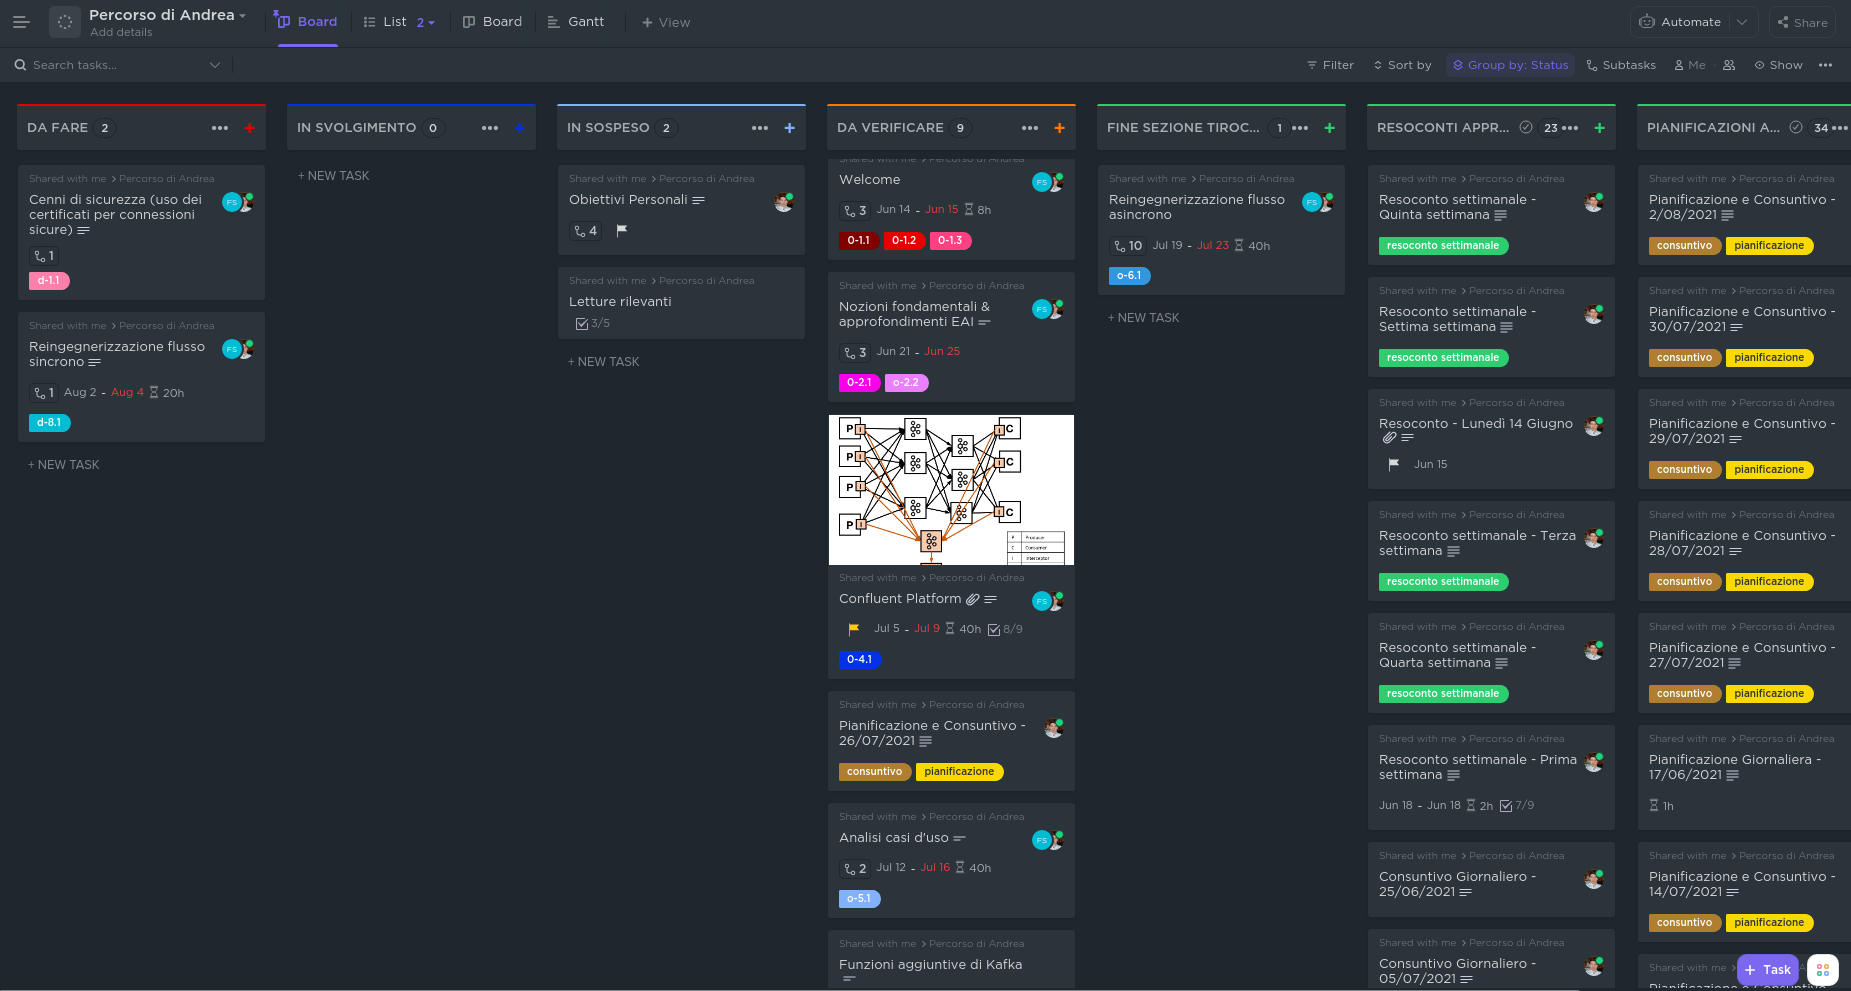
\includegraphics[width=\textwidth]{images/clickup_board.png}\\
  \caption{\textit{Kanban Board} del progetto di \textit{stage}}
\end{figure}
\begin{figure}[h!]
  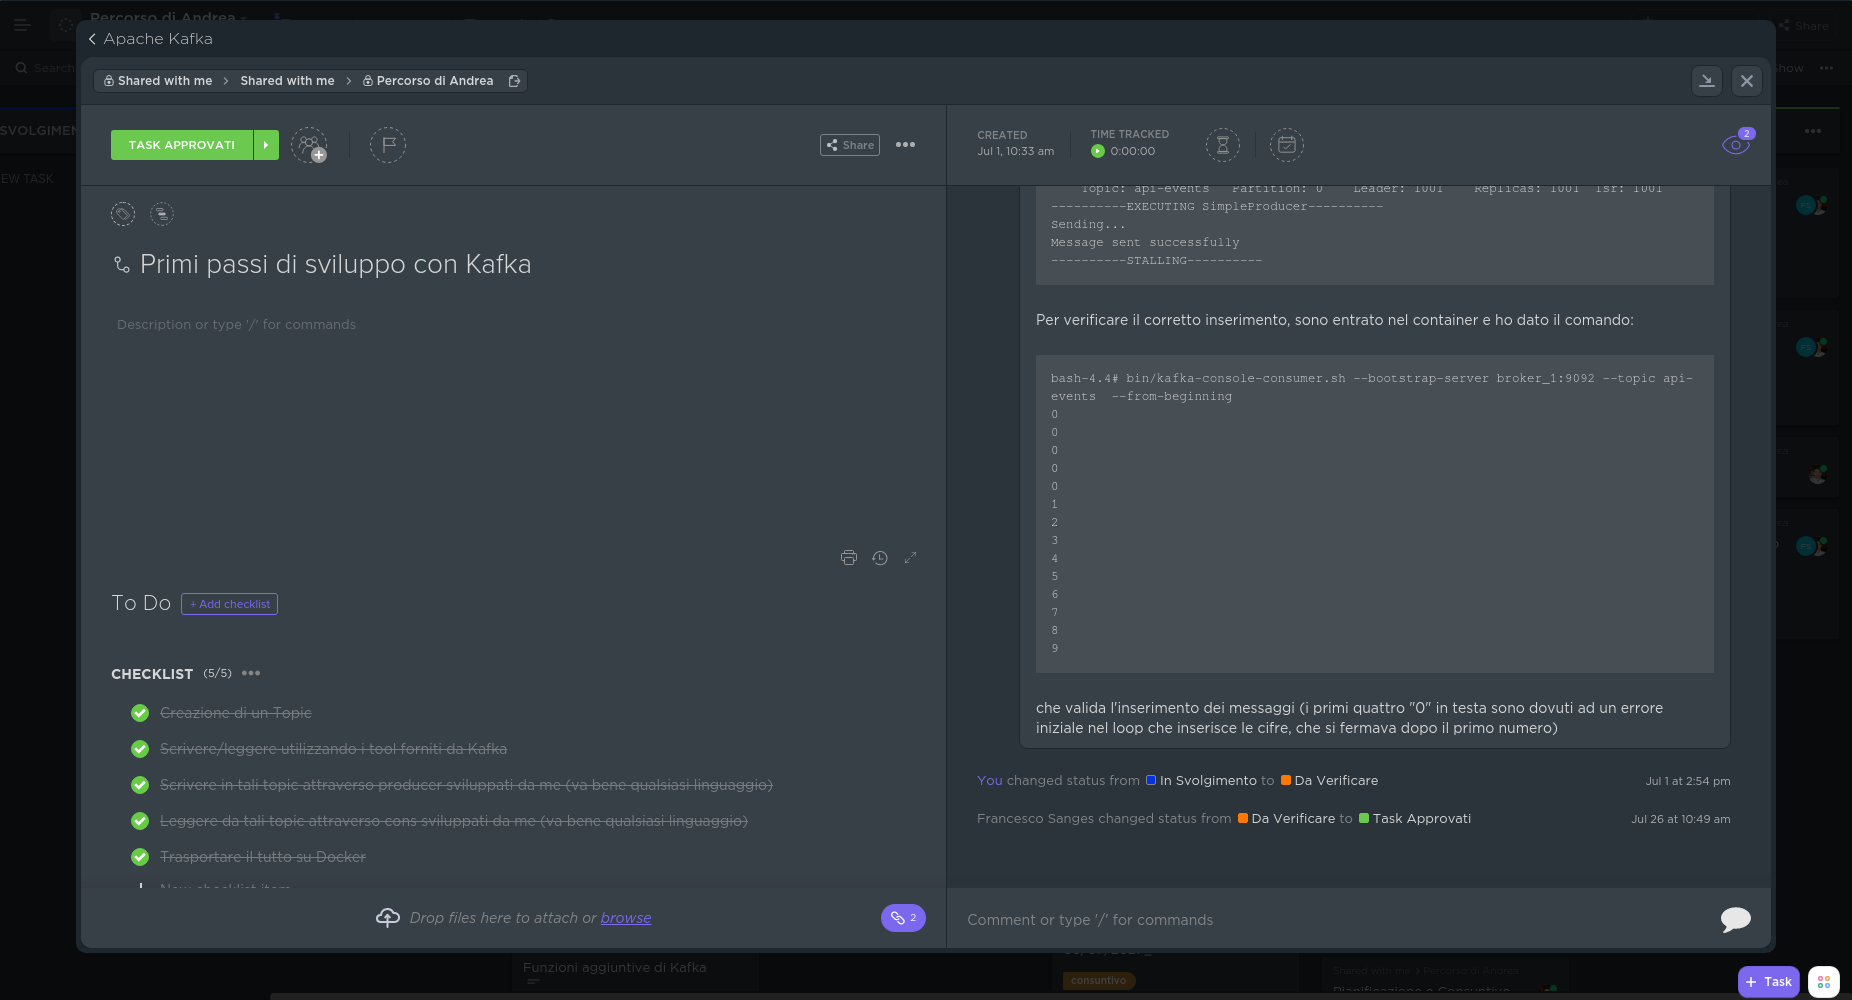
\includegraphics[width=\textwidth]{images/clickup_task.png}\\
  \caption{Esempio di un'attività del processo di Formazione}
\end{figure}

\section{L’ambiente di lavoro}

% Sviluppo indipendente dal sistema operativo, produzione di \textit{software} non strettamente legati ad uno specifico linguaggio, utilizzo di ambienti virtuali quali \textit{Virtual Machine} e \textit{container} per simulare sistemi indipendenti.
L'ambiente di lavoro di cui ho avuto esperienza risulta abbastanza libero e flessibile.
Lo sviluppo del prodotto nell'ambito del EAI dev'essere indipendente dal linguaggio di programmazione, dagli strumenti utilizzati per l'esecuzione e sviluppo, e possibilmente anche dal Sistema operativo su cui eseguire il \textit{software}.
A tal scopo si utilizzano strumenti quali \textit{Virtual Machine} e \textit{Container}: essi non sono garantiscono l'indipendenza dal Sistema Operativo in uso, ma simulano efficacemente il caso d'uso reale in cui i vari eseguibili sono dislocati in più computer o server come spesso accade per il cliente.
Nonostante il percorso formativo abbia visto l'apprendimento di entrambe le tecnologie tramite l'utilizzo dei software \textit{Virtual Box} e \textit{Docker}, infine solo quest'ultima è stata utilizzata durante il progetto poichè più efficente e minimale.

\chapter{Apache Kafka nell’Integrazione Aziendale}

% \section{L'evoluzione delle architetture di integrazione}
\section{Obiettivi aziendali}

Per soddisfare le richieste dei clienti ed essere sempre competitiva e all'avanguardia, una priorità di Sync Lab sono le esplorazioni tecnologiche e di prodotto anche tramite l'utilizzo di percorsi di \stage\ insieme ai laureandi, come quanto accaduto nella mia esperienza.
Questi percorsi consentono all'azienda non solo di testare l'utilizzo di nuovi \software\ ma anche di conoscere e mettere alla prova le capacità del laureando in vista di una potenziale assunzione al termine dello \stage.
\bigskip
% Introduzione al motivo aziendale per cui è nato questo percorso di stage: la propensione odierna alle architetture a microservizi, la gestione di grandi flussi di dati in modo efficiente ed eff1icace, una richiesta di un sistema innovativo da parte della clientela.3

Nel settore dell'\gls{g_eai}, l'evoluzione tecnologica è diretta verso soluzioni sempre più distribuite e con un flusso di dati in continuo aumento.
Uno degli obiettivi specifici nell'area \sacr{eai} di Sync Lab è pertanto quello di trovare un \software\ o tecnologia in grado di soddisfare i bisogni dei clienti di gestire un flusso di dati di dimensioni molto maggiori a quelle attuali, tramite architetture a messaggio che utilizzano servizi distribuiti.

Nell'ambito dei \middleware\ per i sistemi di integrazione, l'aumento del flusso di dati e lo spostamento verso strutture distribuite provoca una difficoltà nella comunicazione e utilizzo di tali dati tra i diversi servizi.
Nell'ambito dell'integrazione per un cliente di piccole dimensioni, in cui i dati circolano tra un numero di componenti limitato, può essere sufficiente un'architetture basata sul \sacrfoot{p2p}.

\begin{figure}[h]
  \begin{center}
    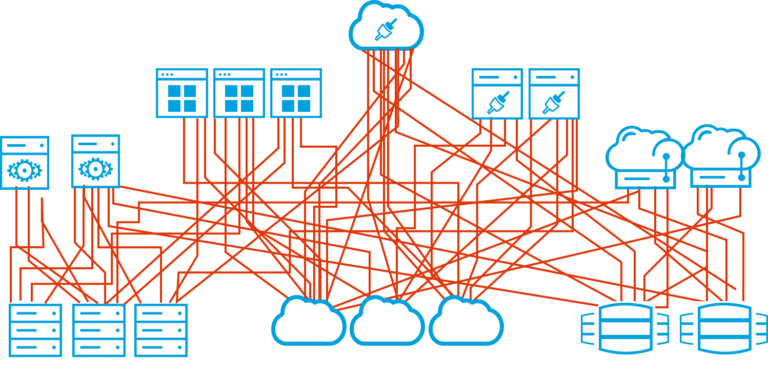
\includegraphics[width=0.8\textwidth]{images/p2p.png}
    \caption{Illustrazione di un sistema basato sul \sacr{p2p}}
    \captionsetup{aboveskip=2pt}
    \caption*{\begin{footnotesize}\textit{Fonte:} \url{https://news.pwc.be/messaging-architecture-with-salesforce/}\end{footnotesize}}
  \end{center}
\end{figure}

Nel caso di un cliente di maggiori dimensioni tuttavia questo approccio rende la manutenzione e gestione del flusso di dati molto difficoltoso e costoso in termini di risorse (figura \thefigure), dato che il grande numero di collegamenti tra i vari punti.

Una delle soluzioni che viene maggiormente implementata per risolvere questo problema è la migrazione verso una \sacr{eda} (\textit{\acrlong{eda}}), un'architettura basata sugli eventi in grado di scambiare dati tra punti multipli.

\begin{figure}[h]
  \begin{center}
    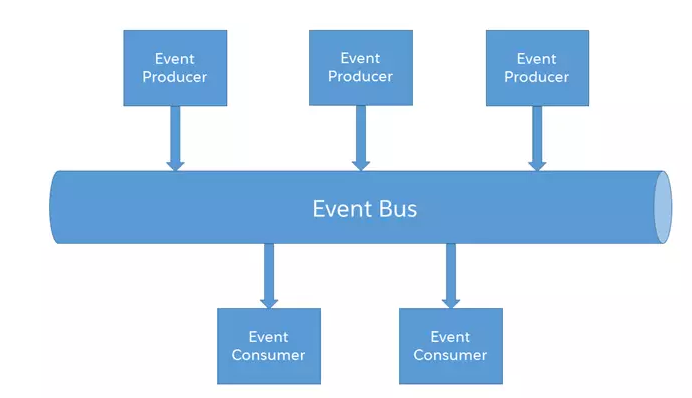
\includegraphics[width=0.8\textwidth]{images/eda.png}
    \caption{Illustrazione di un sistema basato sulla \sacr{eda}}
    \captionsetup{aboveskip=2pt}
    \caption*{\begin{footnotesize}\textit{Fonte:} \url{https://news.pwc.be/messaging-architecture-with-salesforce/}\end{footnotesize}}
  \end{center}
\end{figure}

Questo tipo di architettura è pertanto definita per gestire la produzione, il rilevamento e la reazione agli eventi (figura \thefigure) grazie ad un \textit{Design Pattern} di tipo \textit{Publish/Subscribe}, eliminando i problemi visti precedentemente causati dal sistema \sacr{p2p}.
Questa architettura prevede l'utilizzo di servizi chiamati \textit{Producer}, il cui scopo è fornire dati al \textit{event bus} centrale.
Una volta che i dati sono inseriti all'interno del \textit{bus} centrale, ogni servizio in ascolto (\textit{Subscriber}) li riceverà idealmente in tempo reale.
% \section{L’evoluzione delle architetture di integrazione}
%
% % Introduzione al motivo aziendale per cui è nato questo percorso di stage: la propensione odierna alle architetture a microservizi, la gestione di grandi flussi di dati in modo efficiente ed eff1icace, una richiesta di un sistema innovativo da parte della clientela.3
% L'evoluzione del settore dell'\textit{Enterprise Application Integration} verso soluzioni sempre più distribuite e con un flusso di dati in continuo aumento ha sviluppato nei clienti (e di conseguenza nell'azienda) un interesse verso il prodotto Apache Kafka.
% Il software ha dimostrato negli anni recenti un notevole successo in diversi campi; l'azienda ha interesse nel testare le capacità di Kafka nel soddisfare le esigenze dell'integrazione aziendale.
%
% \bigskip
% \begin{figure}[h]
%   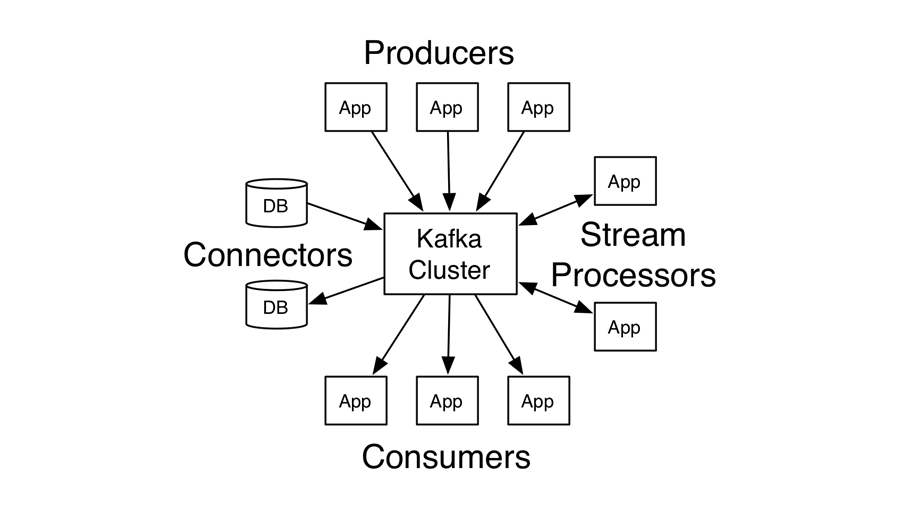
\includegraphics[width=\textwidth]{images/kafka.png}\\
%   \caption{Illustrazione di un sistema a servizi con Apache Kafka}
%   \captionsetup{aboveskip=2pt,font=it}
%   \caption*{Fonte: https://kafka.apache.org/20/documentation.html}
% \end{figure}
%
% Kafka è una piattaforma di \textit{event streaming}, un sistema moderno e distribuito basato sugli eventi anzichè su di una soluzione più classica come può essere quella del \textit{request/response}.
% L'adozione del \software\ nell'ambito dell'EAI è in crescita dato le dimostrate qualità nel gestire grandi moli di dati: la sua performance, sicurezza e scalabilità sono i punti che hanno portato il software al suo attuale successo.
%
% % \bigskip\noindent
% % Esposizioni delle ragioni personali che hanno portato alla scelta di tale percorso.


\subsection{Kafka come Middleware}

Per soddisfare le esigenze di innovazione l'azienda ha avviato un percorso per indagare le capacità del software Apache Kafka nell'ambito dell'integrazione aziendale.

\bigskip
\begin{figure}[h]
  \begin{center}
    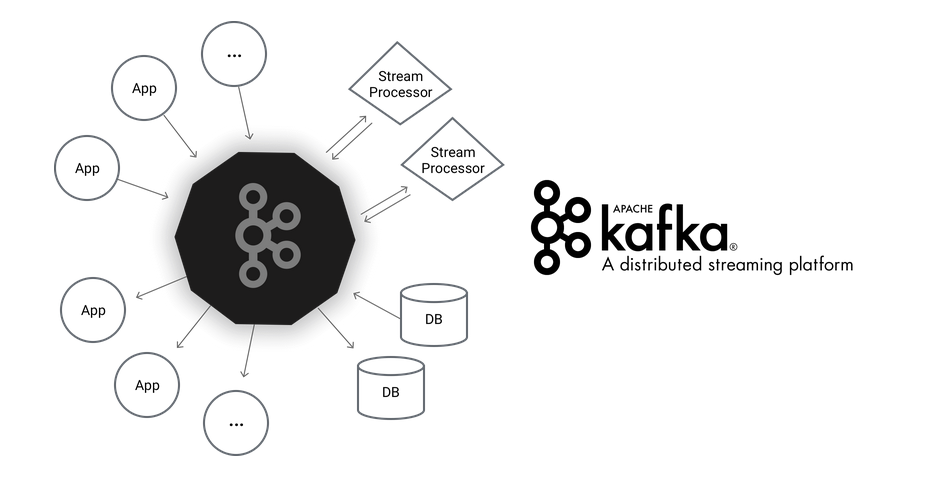
\includegraphics[width=0.45\textwidth, trim={0 0 11.5cm 0},clip]{images/kafka2.png}
    \caption{Illustrazione di Apache Kafka in un caso d'uso esemplificativo}
    \captionsetup{aboveskip=2pt}
    \caption*{\begin{footnotesize}\textit{Fonte:} \url{https://iotbyhvm.ooo/apache-kafka-a-distributed-streaming-platform/}\end{footnotesize}}
  \end{center}
\end{figure}

Apache Kafka si integra ottimamente in molti sistemi basati sul \textit{messaging pattern} e una \sacr{eda}, in cui lo scambio affidabile di dati tra numerosi servizi in tempo reale è essenziale (in figura \thefigure\ è illustrato un caso d'uso esemplificativo di un sistema distribuito basato su Kafka).

% \begin{figure}[h]
%   \begin{center}
%     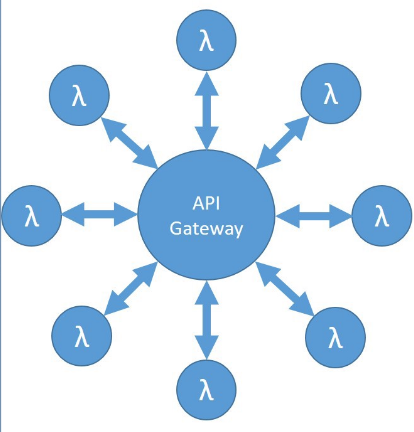
\includegraphics[width=0.35\textwidth, trim={0.07cm 0 0 0},clip]{images/microservices.png}
%     \caption{Illustrazione di un sistema a microservizi con comunicazioni tramite \sacr{api}}
%     \captionsetup{aboveskip=2pt}
%     \caption*{\begin{footnotesize}\textit{Fonte:} \url{https://medium.com/@riyaznet/building-serverless-microservices-on-aws-3959a93c2549}\end{footnotesize}}
%   \end{center}
% \end{figure}

L'interesse di Sync Lab nel \software\ risiede dunque nell'utilizzo di Kafka come un  \textit{Middleware} per soddisfare i problemi di integrazione aziendale e reingegnerizzare i flussi di dati preesistenti, ovvero sviluppare un nuovo sistema che consenta la comunicazione tra differenti servizi con un rapido flusso di dati fra di essi (in figura \thefigure, un semplice sistema a microservizi indipendenti).


L'azienda ha avviato un percorso per testare le capacità di Kafka rispetto agli attuali strumenti utilizzati nel settore, per valutare i vantaggi e svantaggi che l'adozione di tale \software\ può fornire al cliente.

\bigskip\noindent
Sono numerosi i vantaggi che Kafka può portare nel settore, fra cui:
\begin{itemize}
  \item gestione rapida e performante di un enorme flusso di dati;
  \item scalabilità;
  \item sicurezza riguardo la persistenza dei dati;
  \item semplice integrazione e affiancamento a sistemi già esistenti;
  \item l'essere una piattaforma \textit{open source};
  \item processazione dei dati in tempo reale integrata.
\end{itemize}

% \bigskip\noindent
% TODO: Come Kafka possa risolvere i problemi e le necessità viste qui sopra.

\section{Motivazioni e obiettivi personali}

\subsection{Scelta del percorso}

Una delle ragioni che mi ha portato a scegliere questo percorso di \stage\ è l'interesse verso Apache Kafka.
L'utilizzo della piattaforma di \textit{event streaming} è sempre più in crescita, come l'evoluzione verso sistemi sempre più distribuiti e a microservizi.

Un altro fattore fondamentale alla scelta del percorso sono stati la famigliarità con l'azienda, il personale giudizio positivo che ho avuto riguardo il loro metodo di lavoro e la libertà di sviluppo concessa: ho ritenuto importante la possibilità di elaborare personalmente un'architettura del caso d'uso con una visione ad alto livello, anzichè il semplice sviluppo di un software predeterminato e dal percorso strettamente imposto.

\subsection{Obiettivi personali}
L'obiettivo fondamentale dello \stage\ è colmare il divario tra il mondo accademico e quello lavorativo.
Grazie al percorso di \stage\ in una ditta esterna ho avuto l'opportunità di conoscere l'ambiente di lavoro di un'azienda nel campo \sacr{ict}, facilitandomi l'inserimento nel mondo del lavoro.

Un altro obiettivo è ottenere una formazione riguardo la tecnologia di Kafka, che ritengo possa arricchire fortemente le mie capacità e \textit{skill} professionali.
Sono pertanto interessato a sviluppare la mia formazione riguardo l'utilizzo e le implicazioni di questa tecnologia in rapida espansione, la cui formazione potrà essermi utile in molti campi anche al di fuori degli obiettivi dell'azienda ospitante lo \stage.


\section{Il percorso di Stage}


% Descrizione di come il percorso di \textit{stage} si inserisce nella visione più ampia riportata qui sopra.
%
% \bigskip\noindent
% Elenco degli obiettivi del percorso:
% \begin{itemize}
%   \item formazione riguardo Kafka e l’ambito dell’integrazione;
%   \item verificare le capacità di Kafka nell’ambito EAI;
%   \item sperimentare l’utilizzo di Kafka come \textit{Middleware} tramite una simulazione di un caso d’uso reale a servizi indipendenti.
% \end{itemize}
%
% \noindent
% Breve esposizione dei motivi che mi hanno portato a scegliere questo percorso

% TODO:
% - motivazioni riguardo il percorso di stage proposto
% - descrizione del percorso di stage tenendo conto del contesto e degli obiettivi citati sopra
% - descrivere i miei obiettivi rispetto a quelli aziendali
\subsection{Obiettivi dello \textit{stage}}

Il percorso di \textit{stage} offerto dall'azienda si inserisce all'interno della strategia aziendale più ampia descritta sopra.
Al fine di esplorare la tecnologia di Apache Kafka nell'ambito di un \textit{Middleware} per l'integrazione aziendale, l'azienda ha proposto un percorso di \textbf{\textit{stage} il cui obiettivo è la reingegnerizzazione di un flusso di dati asincrono, utilizzando un'architettura basata su Kafka all'interno di un caso d'uso simulato tramite servizi indipendenti.}

\bigskip
Lo stagista ha il compito di osservare, testare e verificare che il \software\ possa svolgere alcuni compiti inerenti all'area del \sacr{eai}, analizzando alcuni casi d'uso presenti in un \textit{Middleware} aziendale in ambito \textit{telco}.
Il percorso di prevede una durata di 300 ore lavorative.

% \bigskip\noindent
% Il percorso proposto prevede le seguenti attività e obiettivi generali:
% \begin{itemize}
%   \item formazione riguardo la piattaforma di \textit{event streaming} Kafka e l'ambito dell'integrazione aziendale;
%   \item verifica delle capacità di Kafka nell'EAI;
%   \item sperimentazione e sviluppo di un \textit{Middleware} basato su Kafka tramite una simulazione di un caso d'uso reale a servizi indipendenti.
% \end{itemize}

\subsection{Prodotti attesi}

\bigskip
\begin{figure}[h]
  \begin{center}
    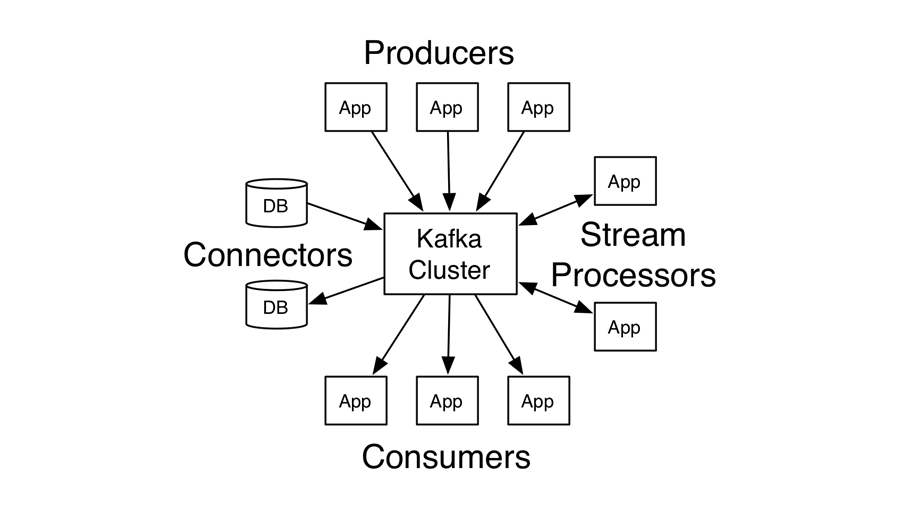
\includegraphics[width=0.8\textwidth]{images/kafka.png}
    \caption{Illustrazione di un sistema a servizi con Kafka}
    \captionsetup{aboveskip=2pt}
    \caption*{\begin{footnotesize}\textit{Fonte:} \url{https://kafka.apache.org/20/documentation.html}\end{footnotesize}}
  \end{center}
\end{figure}

I prodotti attesi al termine dello \textit{stage} sono dunque associati alla realizzazione di tre flussi di integrazione, basati su dei casi d’uso reali, per la gestione dei paradigmi di integrazione asincrono e asincrono con \textit{callback} (due requisiti obbligatori), e sincrono ove fosse disponibile del tempo aggiuntivo e se ritenuto opportuno; durante il percorso considerato il contesto e le opportunità offerte dal \software\ questo obiettivo verrà sostituito per testare delle funzionalità aggiuntive di Kafka.

Il prodotto \software\ finale sarà un sistema basato su servizi indipendenti costruito con un'architettura di tipo \sacr{eda} tramite l'utilizzo di Kafka (figura \thefigure).

\subsection{Contenuti formativi previsti}

La realizzazione di questi prodotti necessita una sostanziale formazione dello stagista riguardo i principali concetti del settore del \textit{Enterprise Application Integration} e l'utilizzo della piattaforma di \textit{event streaming} Kafka.
Più precisamente, i contenuti formativi previsti durante questo percorso di \textit{stage} sono i seguenti:
\begin{itemize}
  \item Concetti chiave del \gls{g_eai};
  \item \textit{Design archittetturali};
  \item Cenni di \textit{Networking} applicato alle architetture distribuite;
  \item Architetture di Integrazione e \textit{Middleware};
  \item Apache Kafka.
\end{itemize}

\subsection{Interazione tra studente e referenti aziendali}
% Personalizzare definendo le modalità di interazione col tutor aziendale
Regolarmente, (almeno una volta la settimana) ci saranno incontri online (tramite la piattaforma Google Meet) con il tutor aziendale Francesco Giovanni Sanges, il responsabile dell’area \sacr{eai} Salvatore Dore e gli esperti delle tecnologie affrontate.
I meeting saranno necessariamente online, dato il dislocamento dei vari membri in diverse città.

Lo scopo di questi incontri sarà quello di verificare lo stato di avanzamento, chiarire gli obiettivi ove necessario, affinare la ricerca e aggiornare la pianificazione iniziale.

\subsection{Pianificazione del lavoro}
\label{sec:pianificazione}
Ad ogni incremento è associato un requisito obbligatorio, desiderabile o facoltativo.
A questi requisiti vi è associato un codice identificativo per favorirne il tracciamento futuro, in che precede la voce descrittiva dell'incremento.
\noindent
Ogni codice è composto da una lettera seguita da dei numeri interi, secondo il seguente modello:
\begin{center}
	\textbf{A-X.Y.Z}
\end{center}
ove, da sinistra verso destra:
\begin{itemize}

  \item \textbf{A} rappresenta la lettera che qualifica il requisito come obbligatorio, desiderabile o facoltativo, secondo la seguente notazione:
  \begin{itemize}
  	\item \textit{O} per i requisiti obbligatori, vincolanti in quanto obiettivo primario richiesto dal committente;
  	\item \textit{D} per i requisiti desiderabili, non vincolanti o strettamente necessari,
  		  ma dal riconoscibile valore aggiunto;
  	\item \textit{F} per i requisiti facoltativi, rappresentanti valore aggiunto non strettamente
  		  competitivo.
  \end{itemize}

  \item \textbf{X} rappresenta la settimana in cui viene inizialmente pianificato l'incremento (identificata da un numero incrementale e intero, partendo da 1).
  Questo consente allo studente, al tutor interno e al tutor interno una rapida quantificazione dell'avanzamento corrente dello stage rispetto a quanto inizialmente pianificato.

  \item \textbf{Y} rappresenta la posizione sequenziale prevista dell’incremento all’interno della settimana (incrementale e intero, partendo da 1). Esso è strettamente associato alla lettera.


\end{itemize}
\noindent
Di seguito viene presentata la pianificazione settimanale delle ore lavorative previste.
Ad ogni settimana sono assegnate le voci contenenti gli incrementi previsti in essa, ove i codici utilizzano la notazione descritta precedentemente.

\noindent
Tutte le settimane prevedono 40 ore lavorative, fatta eccezione per l'ultima che ne prevede 20.

% \usepackage{lscape}
% \newcolumntype{b}{>{\hsize=0.2\textwidth}X}
% \newcolumntype{s}{>{\arraybackslash\hsize=0.2\textwidth}X}
% \newcolumntype{m}{>{\arraybackslash\hsize=0.6\textwidth}X}
\onehalfspacing
\begin{small}
  \begin{center}
    \centering
    \renewcommand\arraystretch{1.6}
    \begin{longtable}{| >{\centering\arraybackslash}m{2cm}|m{1.2cm}|m{10.5cm}|}
      \hline
      \textsc{\textbf{Settimana}} & \textsc{\textbf{Codice}} & \textsc{\textbf{Task associati}} \\
      \hline

      \multirow{8}{*}{\normalsize\textbf{1}}
      & \centering O-1.1 & Incontro con le persone coinvolte nel progetto per discutere i requisiti e le richieste relative al sistema da sviluppare\\
      \cline{2-3}
      & \centering O-1.2 & Verifica credenziali e strumenti di lavoro assegnati\\
      \cline{2-3}
      & \centering O-1.3 & Presa visione dell’infrastruttura esistente\\
      \cline{2-3}
      & \centering D-1.1 & Ripasso approfondito riguardo i seguenti argomenti:
      \smallskip
        \begin{itemize}
           \item Ingegneria del \software;
           \item Sistemi di versionamento;
           \item Architetture \software;
           \item Cenni di \textit{Networking}.
         \end{itemize} \\
     \Xhline{2\arrayrulewidth}

      \multirow{8}{*}{\normalsize\textbf{2}}
      & \centering O-2.1 & Nozioni fondamentali riguardo \sacr{eai} e \sacrfoot{soa}\\
      \cline{2-3}
      & \centering O-2.2 & Approfondimenti riguardo le Architetture a Messaggio, in particolare:
        \begin{itemize}
           \item \textit{Integration Styles};
           \item \textit{Channel Patterns};
           \item \textit{Message Construction Patterns};
           \item \textit{Routing Patterns};
           \item \textit{Transformation Patterns};
           \item \textit{System Management Patterns}.
         \end{itemize} \\
     \Xhline{2\arrayrulewidth}

      \multirow{2}{*}{\normalsize\textbf{3}}
      & \centering O-3.1 & Apache Kafka:
        \begin{itemize}
            \item Introduzione a Kafka;
            \item Concetti fondamentali di Kafka;
            \item Avvio e \sacrfoot{cli};
            \item Programmazione in Kafka con Java.
          \end{itemize} \\
      \cline{2-3}
      & \centering D-3.1 & Esempi e applicazioni di Apache Kafka \\
     \Xhline{2\arrayrulewidth}

     \multirow{1}{*}{\normalsize\textbf{4}}
     & \centering O-4.1 & Confluent Platform:
       \begin{itemize}
         \item \textit{Service registry};
         \item \sacr{rest} \textit{proxy};
         \item kSQL;
         \item Confluent \textit{connectors};
         \item \textit{Control center}.
       \end{itemize} \\
    \Xhline{2\arrayrulewidth}

    \multirow{2}{*}{\normalsize\textbf{5}}
    & \centering O-5.1 & Analisi dei casi d'uso reali\\
    \cline{2-3}
    & \centering O-5.2 & Realizzazione dei componenti per l'esecuzione dei casi di test\\
    \Xhline{2\arrayrulewidth}

    \multirow{1}{*}{\normalsize\textbf{6}}
    & \centering O-6.1 & Analisi reingegnerizzazione e collaudo del flusso di integrazione asincrono\\
    \Xhline{2\arrayrulewidth}

    \multirow{1}{*}{\normalsize\textbf{7}}
    & \centering O-7.1 & Analisi e reingegnerizzazione e collaudo del flusso di integrazione asincrono con callback\\
    \Xhline{2\arrayrulewidth}

    \multirow{1}{*}{\normalsize\textbf{8}}
    & \centering O-8.1 & Analisi e reingegnerizzazione e collaudo del flusso di integrazione sincrono\\
    \hline
    \caption{Pianificazione settimanale dello \textit{stage}}
    \label{tab:pianificazione}
    \end{longtable}
  \end{center}
\end{small}
\doublespacing

% \begin{table}
%  \begin{tabularx}{\textwidth}{X*{5}{>{\centering\arraybackslash}X}}
%  \hline
%  Sample window & Probability cutoff value & Crises Correctly called (\%) &
%  Non-crises correctly called (\%) & Missed crises & False Alarm  \\
%  \hline
% \end{tabular}
% \end{table}
%
% \begin{itemize}
%        \item \textbf{Prima Settimana (40 ore)}
%        \begin{itemize}
%            \item \textbf{O-1.1} Incontro con le persone coinvolte nel progetto per discutere i requisiti e le richieste relative al sistema da sviluppare;
%            \item \textbf{O-1.2} Verifica credenziali e strumenti di lavoro assegnati;
%            \item \textbf{O-1.3} Presa visione dell’infrastruttura esistente;
%            \item \textbf{D-1.1} Ripasso approfondito riguardo i seguenti argomenti:
%              \begin{itemize}
%                \item Ingegneria del \software;
%                \item Sistemi di versionamento;
%                \item Architetture \software;
%                \item Cenni di \textit{Networking}.
%              \end{itemize}
%        \end{itemize}
%
%        \item \textbf{Seconda Settimana (40 ore)}
%        \begin{itemize}
%            \item \textbf{O-2.1} Nozioni fondamentali riguardo \sacr{eai} e \sacrfoot{soa};
%            \item \textbf{O-2.2} Approfondimenti riguardo le Architetture a Messaggio, in particolare:
%              \begin{itemize}
%                \item \textit{Integration Styles};
%                \item \textit{Channel Patterns};
%                \item \textit{Message Construction Patterns};
%                \item \textit{Routing Patterns};
%                \item \textit{Transformation Patterns};
%                \item \textit{System Management Patterns}.
%              \end{itemize}
%        \end{itemize}
%
%        \item \textbf{Terza Settimana (40 ore)}
%        \begin{itemize}
%            \item \textbf{O-3.1} Apache Kafka:
%              \begin{itemize}
%                \item Introduzione a Kafka;
%                \item Concetti fondamentali di Kafka;
%                \item Avvio e \sacrfoot{cli};
%                \item Programmazione in Kafka con Java.
%              \end{itemize}
%            \item \textbf{D-3.1} Esempi e applicazioni di Apache Kafka.
%        \end{itemize}
%
%
%        \item \textbf{Quarta Settimana (40 ore)}
%        \begin{itemize}
%            \item \textbf{O-4.1} Confluent Platform:
%              \begin{itemize}
%                \item Service registry;
%                \item REST proxy;
%                \item kSQL;
%                \item Confluent connectors;
%                \item Control center.
%              \end{itemize}
%        \end{itemize}
%
%        \item \textbf{Quinta Settimana (40 ore)}
%        \begin{itemize}
%          \item \textbf{O-5.1} Analisi dei casi d'uso reali;
%          \item \textbf{O-5.2} Realizzazione dei componenti per l'esecuzione dei casi di test.
%        \end{itemize}
%
%        \item \textbf{Sesta Settimana (40 ore)}
%        \begin{itemize}
%          \item \textbf{O-6.1} Analisi reingegnerizzazione e collaudo del flusso di integrazione asincrono.
%        \end{itemize}
%
%        \item \textbf{Settima Settimana (40 ore)}
%        \begin{itemize}
%            \item \textbf{O-7.1} Analisi e reingegnerizzazione e collaudo del flusso di integrazione asincrono con callback
%
%        \end{itemize}
%
%        \item \textbf{Ottava Settimana (20 ore)}
%        \begin{itemize}
%            \item \textbf{D-8.1} Analisi e reingegnerizzazione e collaudo del flusso di integrazione sincrono.
%        \end{itemize}
%
% \end{itemize}

\begin{figure}[h]
  \begin{center}
    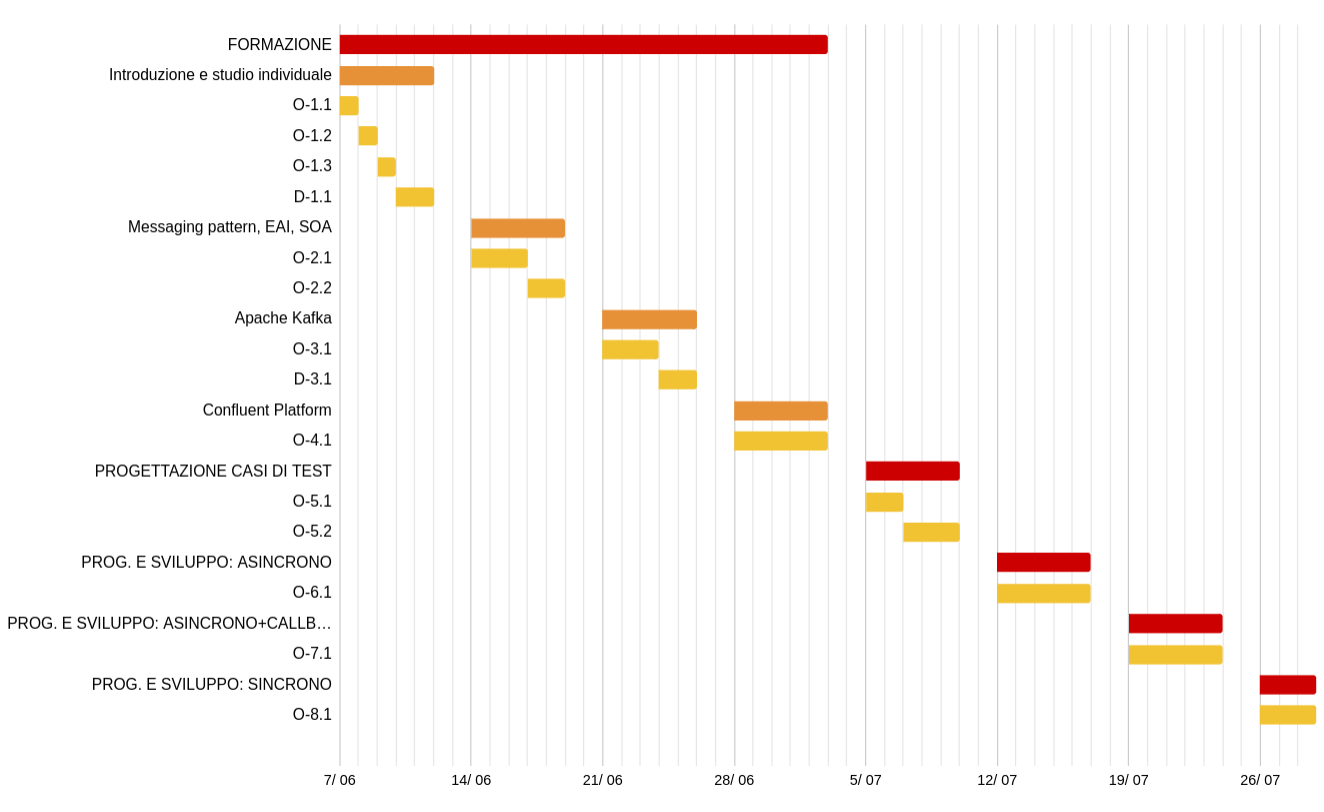
\includegraphics[width=\textwidth]{images/gantt.png}
    \caption{Diagramma di Gantt del piano di lavoro}
    \captionsetup{aboveskip=2pt}
    \caption*{\begin{footnotesize}\textit{Fonte: elaborazione personale}\end{footnotesize}}
  \end{center}
\end{figure}

\noindent
Secondo questa pianificazione, (di cui la figura \thefigure\ rappresenta il diagramma di Gantt) le 300 ore di \stage\ previste sono approsimativamente divise in:
\begin{itemize}
  \item 160 ore di Formazione sulle tecnologie;
  \item 60 ore di Progettazione dei componenti e dei test;
  \item 60 ore di Sviluppo dei componenti e dei test;
  \item 20 ore di Valutazioni finali, Collaudo e Presentazione della Demo.
\end{itemize}

% \chapter{Apache Kafka in caso d’uso simulato}
\chapter{Il percorso di stage}

\section{Formazione}

Il processo di Formazione ha avuto un importante ruolo all'interno dello \textit{stage}, con una durata complessiva di circa quattro settimane.
La causa di questo lungo periodo di formazione è data dallo studio di diversi ambiti e concetti per me nuovi, in particolare il settore del \textit{\acrlong{eai}} e la tecnologia di Kafka.

% \bigskip
\begin{figure}[h]
  \begin{center}
    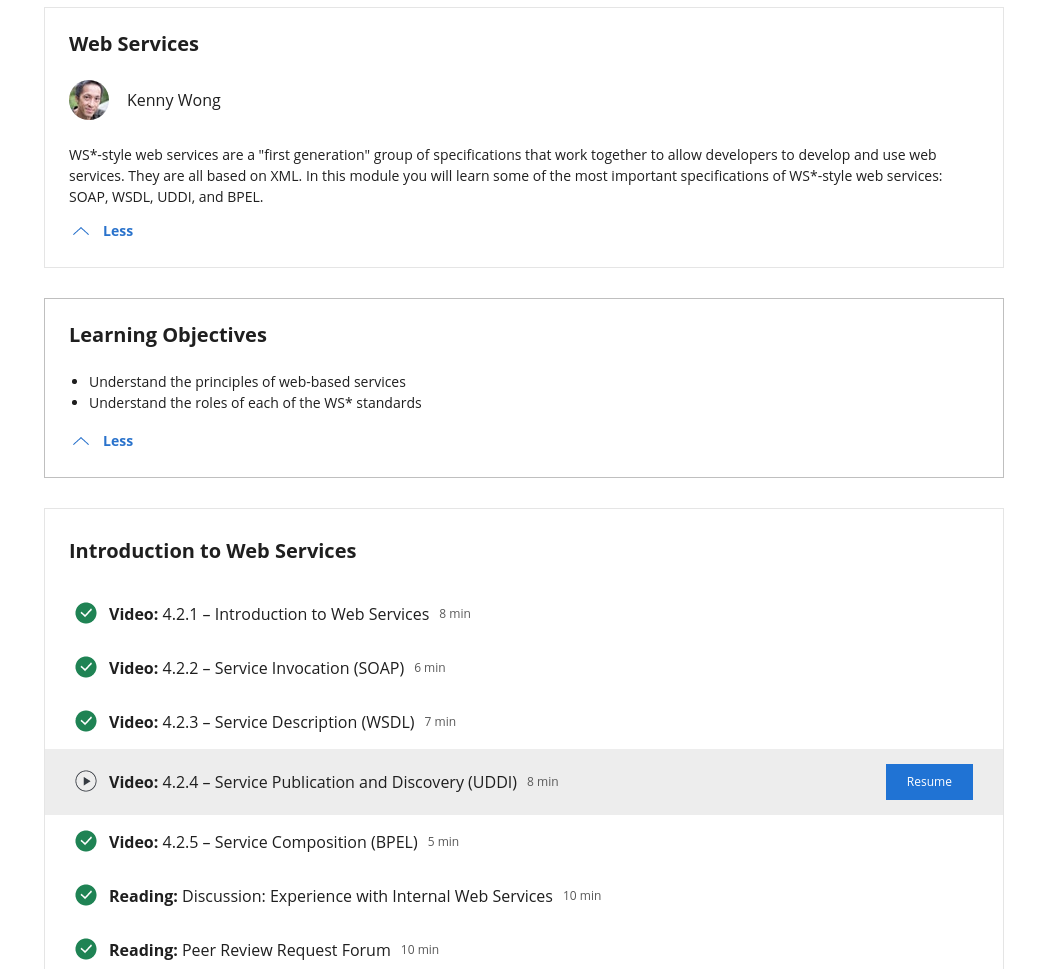
\includegraphics[width=0.7\textwidth]{images/coursera_week2.png}
    \caption{Screenshot del corso online \textit{acrlong{soa}} sulla piattaforma Coursera}
    \captionsetup{aboveskip=2pt}
    \caption*{\begin{footnotesize}\textit{Fonte: elaborazione personale}\end{footnotesize}}
  \end{center}
\end{figure}


Durante questo processo Sync Lab mi ha fornito del materiale didattico per l'apprendimento, quali diapositive e appunti di origine aziendale e l'accesso a dei corsi riguardo \textit{Software architecture}, \textit{\acrlong{soa}} (figura \thefigure) (tramite i corsi online su \textit{Coursera}) e Apache Kafka (tramite i corsi online su \textit{Udemy}).

Il tutor aziendale e responsabile \sacr{eai} hanno fornito durante i \textit{meeting} settimanali ulteriori chiarimenti e approfondimenti sul come Sync Lab applica questi concetti nello sviluppo di architetture \software.

Per i corsi online a maggiore contenuto nozionistico ho redatto degli appunti riassuntivi, con lo scopo di consolidare l'apprendimento e velocizzare la verifica del tutor aziendale.

\section{Analisi e modellazione di un caso d'uso}

Ad alcune videoconferenze ha partecipato anche un esperto \textit{senior} aziendale, esterno al progetto di \stage\ in questione, per illustrarmi un caso d'uso in cui l'azienda ha esposto un prototipo di sistema di integrazione utilizzando i concetti di \textit{Web Service}, \sacrfoot{soap} e \textit{request/response}, permettendomi la visualizzazione dei file \sacrfoot{wsdl}, \sacrfoot{xml} e \sacrfoot{xsd} associati.
Ho pertanto generato un caso d'uso adatto agli scopi dello \stage\ ispirandomi al caso d'uso reale illustrato.

Il caso d'uso modellato tratta una richiesta di credito telefonico da parte di un cliente ad un'azienda di telecomunicazioni tramite \textit{Web Service}, per soddisfare il requisito dello sviluppo della re-ingegnerizzazione del flusso di dati asincrono.
La \textit{request} avviene tramite flusso di un file \sacrfoot{json} che viene trasmesso attraverso i vari servizi che compongono il sistema di integrazione, basato sul \textit{Design Pattern} di tipo \textit{publish/subscribe}.

Va precisato che il contenuto di tale \sacr{json} non è strettamente rilevante allo sviluppo e funzionamento del \textit{Middleware}, ma aiuta a stabilire il contesto di utilizzo.

% \bigskip
% \begin{figure}[h]
%   \begin{center}
%     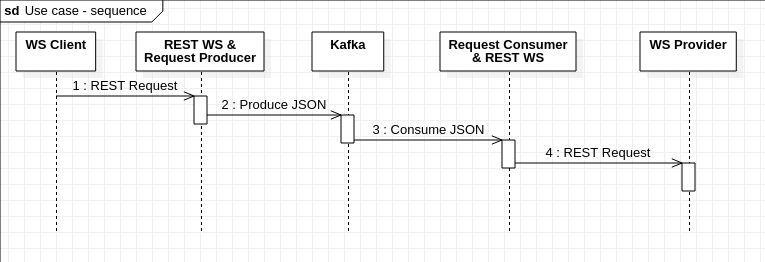
\includegraphics[width=\textwidth, trim={0.08cm 0 0 0.08cm},clip]{images/uc_sequence.png}
%     \caption{Diagramma di sequenza \sacr{uml} per il prototipo di caso d'uso iniziale}
%     \captionsetup{aboveskip=2pt}
%     \caption*{\begin{footnotesize}\textit{Fonte: elaborazione personale}\end{footnotesize}}
%   \end{center}
% \end{figure}

\noindent
Il caso d'uso è composto dai seguenti passaggi:
\begin{enumerate}
  \item il cliente (\textit{\sacrfoot{ws} Client}) effettua una richiesta di credito tramite invio di un file \sacr{json} al successivo Servizio Web in ascolto.
  \item il servizio composto da \sacrfoot{rest} \sacr{ws} e \textit{Request Producer} riceve il \sacr{json} e lo inserisce in Kafka tramite l'apposito \textit{Kafka Producer}, assumendo la funzione di \textit{publisher}.
  \item il servizio di \textit{Request Consumer}, sottoscritto al \textit{topic} in questione riceve il \sacr{json} e lo invia al \sacr{ws} finale tramite una \sacr{rest} request.
  \item il servizio in coda chiamato \sacr{ws} \textit{Provider} riceve il \sacr{json}; grazie ai dati ricevuti è in grado di fornire il servizio richiesto dal \textit{Client} nello \textit{step} 1.
\end{enumerate}

La modellazione dell'architettura e struttura del sistema da sviluppare seguirà questo prototipo di \sacrfoot{uc}.
Il modello associato al caso asincrono con \textit{callback} seguirà la stessa struttura e \textit{step} dello \sacr{uc} illustrato qui sopra, con l'aggiunta speculare del messaggio di ritorno.

\section{Progettazione architetturale}\label{sec:progettazione}
\subsection{Un \textit{middleware} basato su un \sacr{eda}}

La progettazione architetturale ha portato alla produzione di diversi diagrammi \sacr{uml} per rappresentare efficacemente l'architettura del prodotto e fornire un modello da seguire durante il processo di codifica.
Il processo ha richiesto frequenti \textit{meeting} e confronti per raggiungere un risultato finale soddisfacente al fine della sperimentazione.

La progettazione architetturale del prodotto comprende un \middleware\ centrale basato su di una \textit{\acrlong{eda}} con l'utilizzo di Apache Kafka, e due componenti di \textit{testing} chiamati \textit{service client} e \textit{service provider}, che simulano due servizi esterni che comunicano con il middleware attraverso \sacr{rest} \textit{request}.

Il sistema è composto da molteplici microservizi, che comunicano attraverso la rete di Docker.
L'obiettivo della progettazione è modellare un \middleware\ che sia implementabile in una \textit{\acrlong{soa}}, e consentirne la verifica e collaudo grazie ai servizi di \textit{testing}.

\begin{figure}[H]
  \begin{center}
    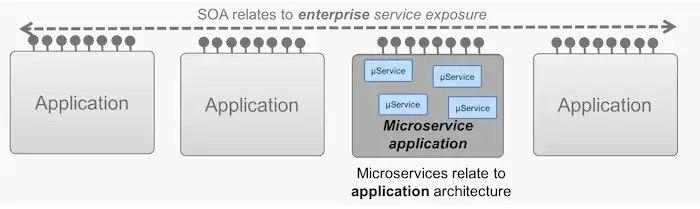
\includegraphics[width=0.7\textwidth]{images/soa_vs_micro.jpg}
    \caption{Visione ad alto livello delle differenze tra \sacr{soa} e microservizi}
    \captionsetup{aboveskip=2pt}
    \caption*{\begin{footnotesize}\textit{https://www.ibm.com/cloud/blog/soa-vs-microservices}\end{footnotesize}}
  \end{center}
\end{figure}

In figura \thefigure\ è rappresentata una visione ad alto livello dell'implementazione di un'applicazione a microservizi all'interno di una \sacr{soa}, evidenziando la differenza tra i due concetti.
% \bigskip

Per rappresentare in modo chiaro ed elegante il modello descritto dal \sacr{uc} sopra, ho elaborato diversi diagrammi \sacr{uml}.
% I diagrammi di maggiore rilevanza, oltre ad essere esposti all'interno di questa sezione accanto alla spiegazione associata, sono allegati in formato più grande a
Questi diagrammi rappresentano i componenti \textit{color coded}, notazione utilizzata per dare continuità e chiarezza attraverso le diverse tipologie di \sacr{uml} \textit{diagrams}.

\subsection{\sacr{uml} \textit{sequence diagrams}}

% \begin{figure}[H]
%   \begin{center}
%     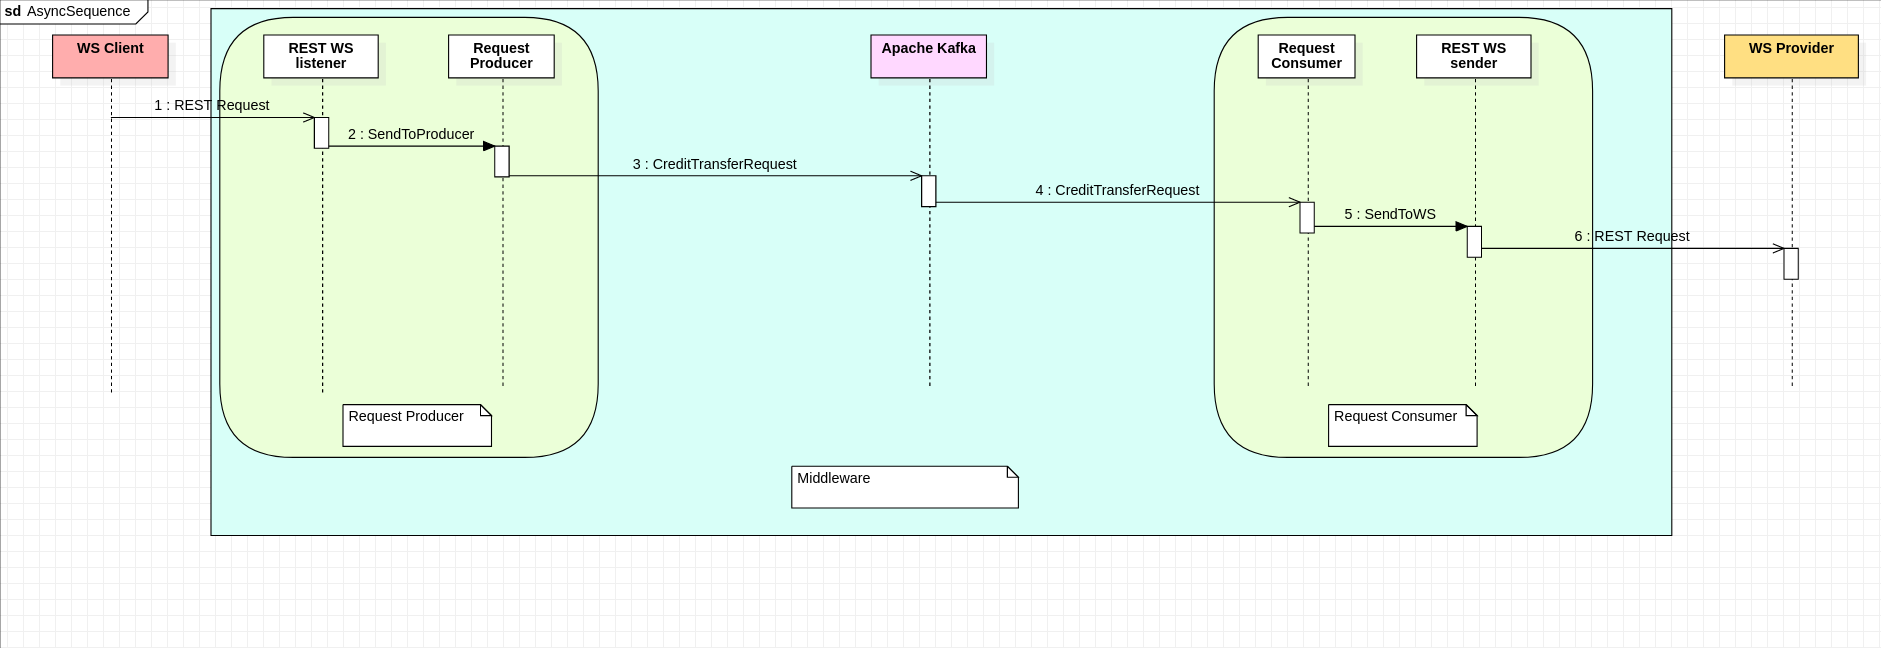
\includegraphics[width=\textwidth, trim={0.2cm 0 0 0.2cm},clip]{images/a_sequence2.png}
%     \caption{Diagramma \sacr{uml} di sequenza per la reingegnerizzazione del flusso asincrono}
%     \captionsetup{aboveskip=2pt}
%     \caption*{\begin{footnotesize}\textit{Fonte: elaborazione personale}\end{footnotesize}}
%   \end{center}
% \end{figure}

A partire dallo \sacr{uc} descritto nella sezione precedente, ho prodotto un \sacr{uml} \textit{sequence diagram} più approfondito per rappresentare il flusso del \sacr{json} tra i vari componenti.
% (figura \thefigure).

% \begin{figure}[h]
%   \begin{center}
%     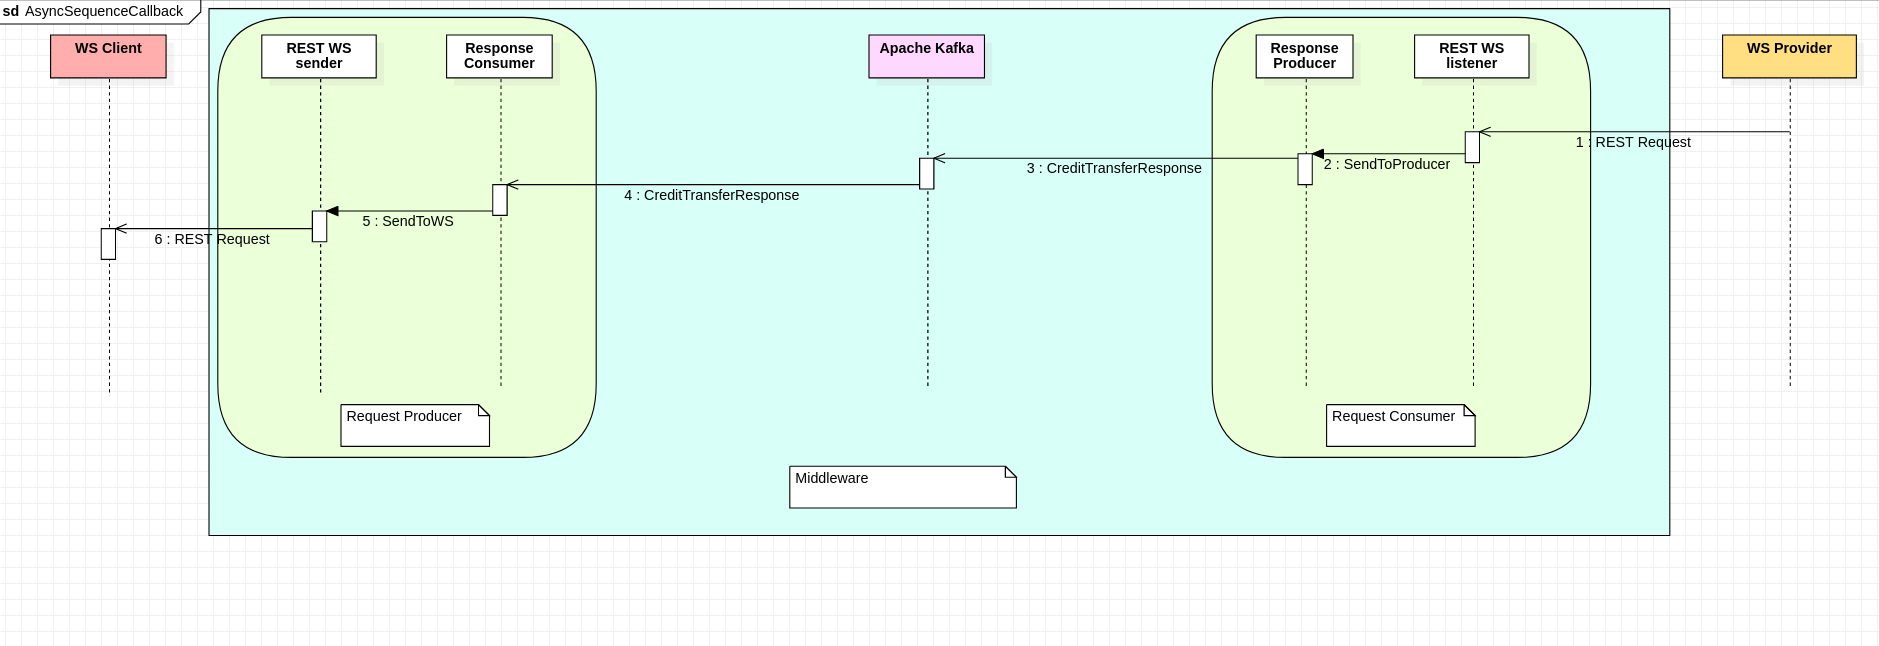
\includegraphics[width=\textwidth]{images/ac_sequence.png}
%     \caption{Diagramma di sequenza \sacr{uml} per la reingegnerizzazione del flusso asincrono con \textit{callback}}
%     \captionsetup{aboveskip=2pt}
%     \caption*{\begin{footnotesize}\textit{Fonte: elaborazione personale}\end{footnotesize}}
%   \end{center}
% \end{figure}

La progettazione del sistema associato al caso asincrono con \textit{callback} comprende lo stesso schema \sacr{uml} del caso asincrono, con aggiunta del flusso di ritorno speculare flusso di andata
% descritto nella figura \thefigure.

La re-ingegnerizzazione del flusso sincrono è stata scartata in favore dello studio di funzionalità aggiuntive tramite l'utilizzo della piattaforma di \textit{event streaming}.
La progettazione di un sistema basato su questo flusso era inizialmente prevista (come requisito desiderabile) nel piano di lavoro iniziale poiché associata ad un caso d'uso reale (di cui si è parlato nelle sezioni precedenti), ma infine è stata giudicata poco opportuna e fuori dagli scopi di Apache Kafka, un sistema basato sull'asincronismo.

Il tempo associato a tale requisito è stato pertanto riproposto per testare un'altra funzione utile in un \middleware\, quali la trasformazione di alcuni dati presenti nel \sacr{json}.
Più precisamente, è stato aggiunto un dato sensibile che viene nascosto e sostituito con asterischi "*" dopo la produzione del \textit{topic} in Kafka grazie all'utilizzo di Kafka Streams.
% \bigskip
\begin{figure}[h]
  \begin{center}
    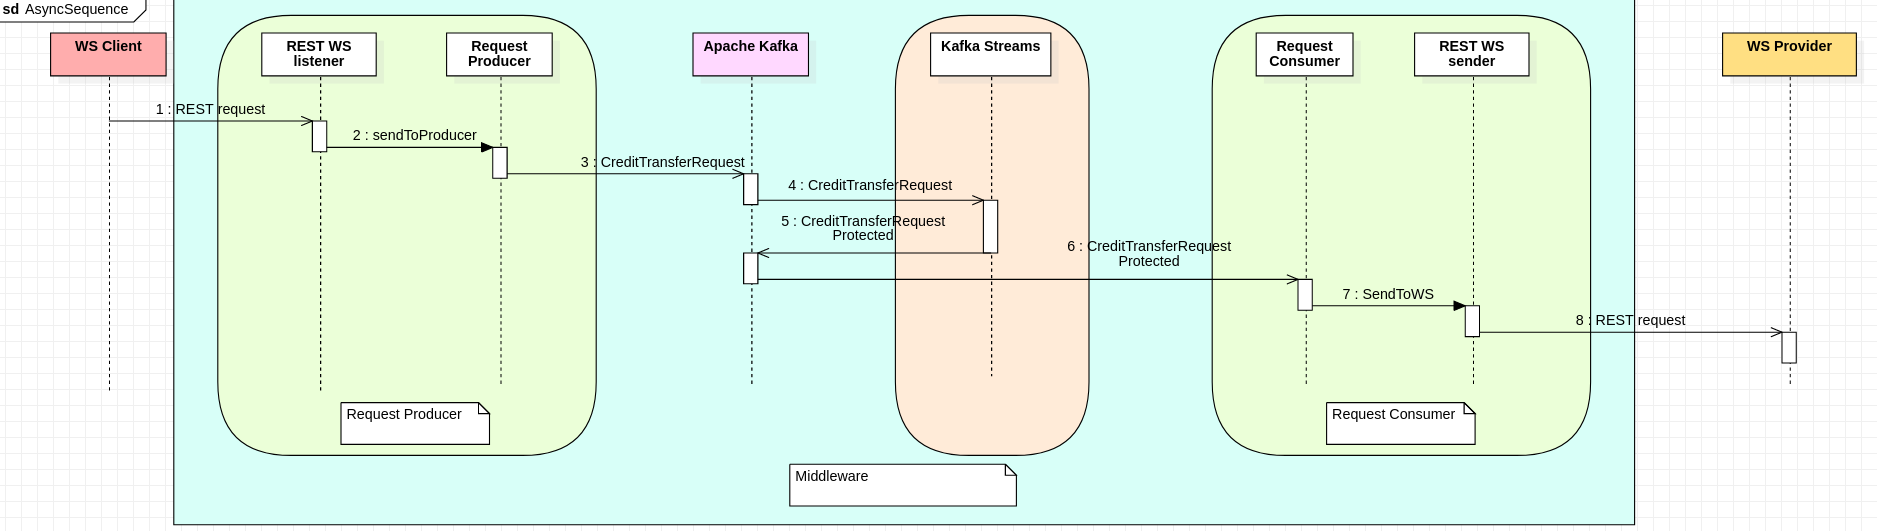
\includegraphics[width=\textwidth]{images/ap_sequence.png}
    \caption{Diagramma di sequenza \sacr{uml} per la re-ingegnerizzazione del flusso asincrono con protezione dei dati sensibili.}
    \captionsetup{aboveskip=2pt}
    \caption*{\begin{footnotesize}\textit{Fonte: elaborazione personale}\end{footnotesize}}
  \end{center}
\end{figure}

In figura \thefigure\ possiamo vedere il nuovo flusso asincrono con protezione (mascheramento) del dato sensibile.
La versione con \textit{callback} del flusso qui sopra prevede anche il flusso di ritorno (\textit{callback}), non illustrato in figura ma facilmente intuibile grazie al grafico che la precede.

\subsection{\sacr{uml} \textit{deployment diagram}}
\label{sub:uml_deployment}

A supporto di questi \sacr{uml} \textit{sequence diagram} che rappresentano efficacemente il flusso di dati, punto focale dell'intero sistema di integrazione (asincrono con la protezione del dato sensibile), ho prodotto ulteriori diagrammi, tra i quali il \textit{deployment diagram}.

\begin{figure}[h]
  \begin{center}
    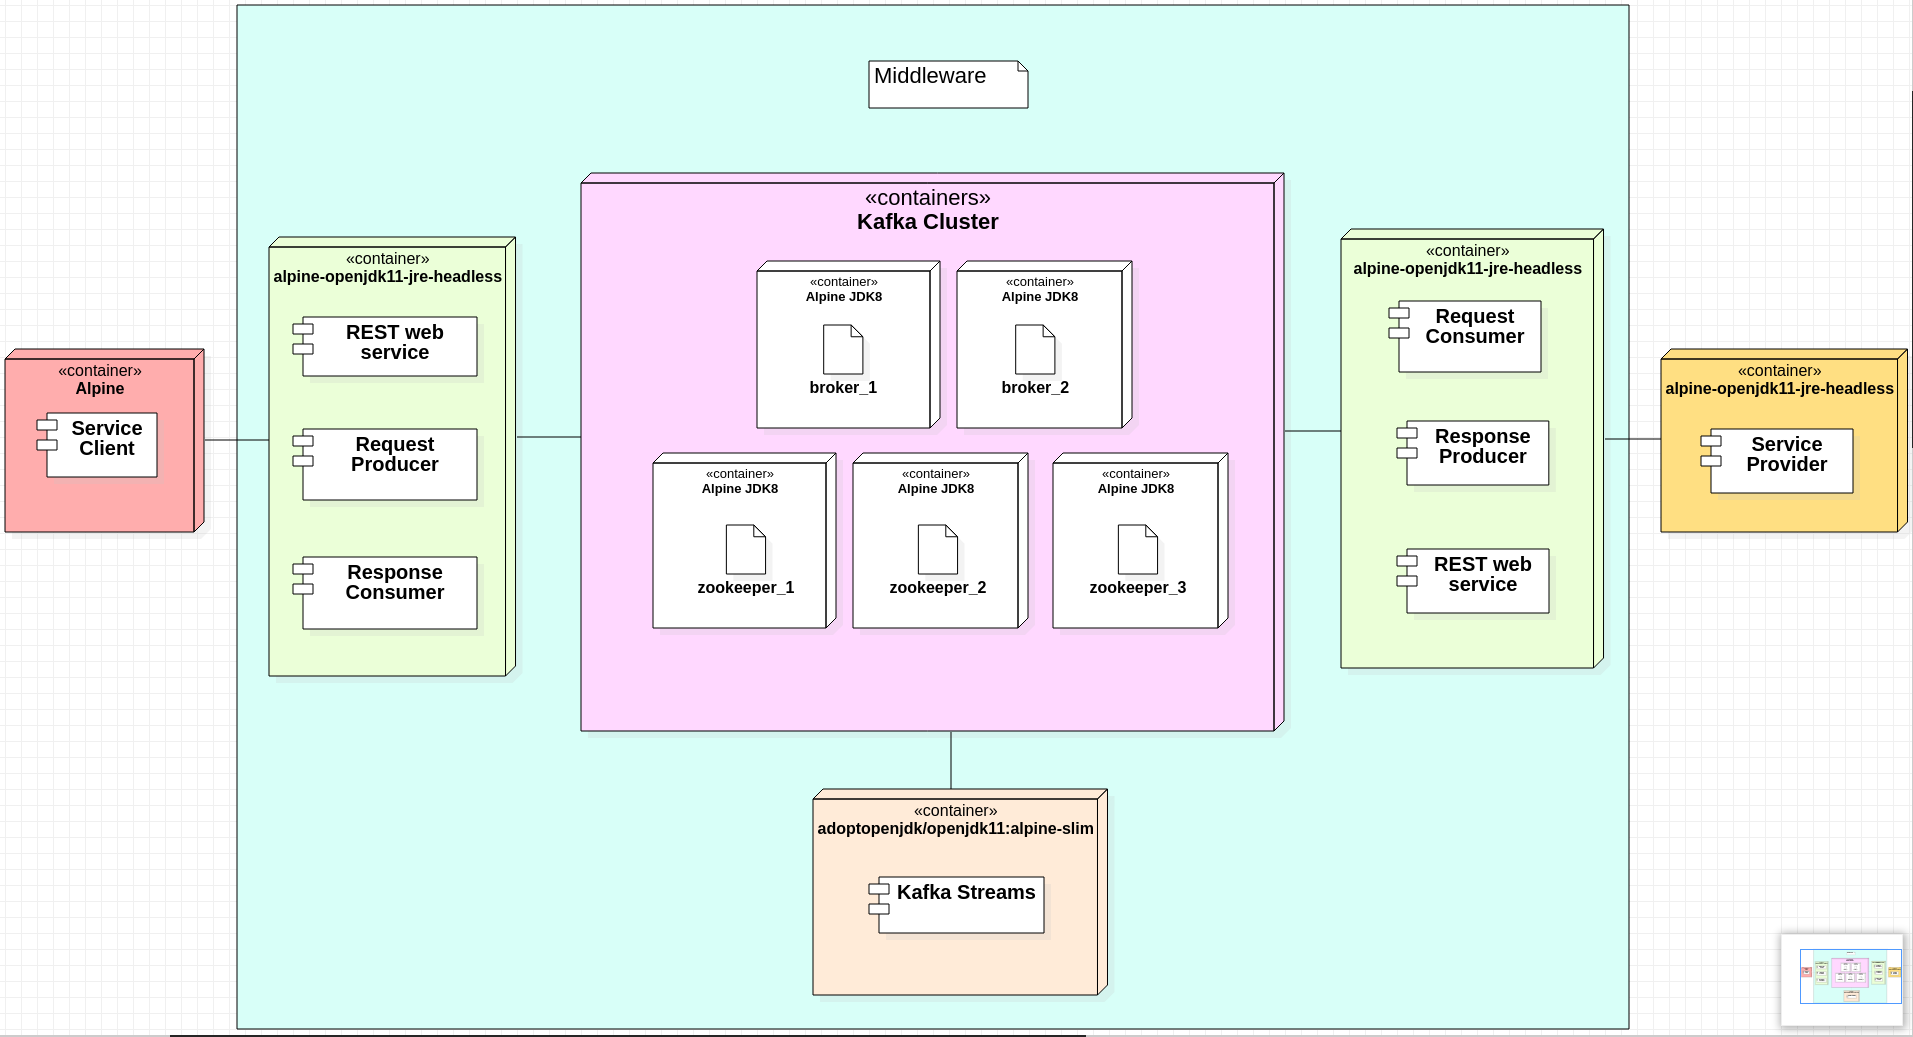
\includegraphics[width=\textwidth,  trim={0 0.2cm 0.2cm 0},clip]{images/ap_deployment.png}
    \caption{\sacr{uml} \textit{deployment diagram} per la re-ingegnerizzazione del flusso asincrono (protetto)}
    \captionsetup{aboveskip=2pt}
    \caption*{\begin{footnotesize}\textit{Fonte: elaborazione personale}\end{footnotesize}}
  \end{center}
\end{figure}

Questo diagramma (figura \thefigure) ha lo scopo di rappresentare la configurazione dei processi \textit{run time}, modellando la struttura di base in cui eseguono i diversi servizi;
il diagramma esprime l'ambiente in cui i vari componenti risiedono e ove essi comunicano tra di loro.

Con l'approvazione degli esperti aziendali, ho deciso di appoggiare il sistema di integrazione sulla piattaforma Docker.

Il diagramma di \textit{deployment} vede pertanto l'utilizzo di numerosi \textit{container} indipendenti che dialogano attraverso una rete locale all'interno di Docker.
Questi \textit{container} sono raffigurati dai vari nodi (rappresentati dai cubi in rilievo in figura).
A questa notazione fa eccezione il nodo virtuale intitolato "Kafka Cluster", che ha solamente lo scopo di raggruppare i vari nodi legati al \textit{environment} di Kafka con funzione comune, ma che in realtà non compone un container reale a se stante.
All'interno di questi nodi sono rappresentati gli artefatti che eseguono nel relativo \textit{container}, per esplicitare la presenza dei componenti.
Si può inoltre notare che l'ambiente di Apache Kafka è composto da un \textit{cluster} composto da due servizi \textit{Broker} e tre servizi \textit{Zookeeper}, allo scopo di simulare un caso d'uso reale in cui i diversi componenti sono distribuiti in sistemi indipendenti e garantiscono l'affidabilità dello \textit{streaming} di eventi.

\subsection{\sacr{uml} \textit{component diagram}}
\label{sub:uml_component}

\begin{figure}[H]
  \begin{center}
    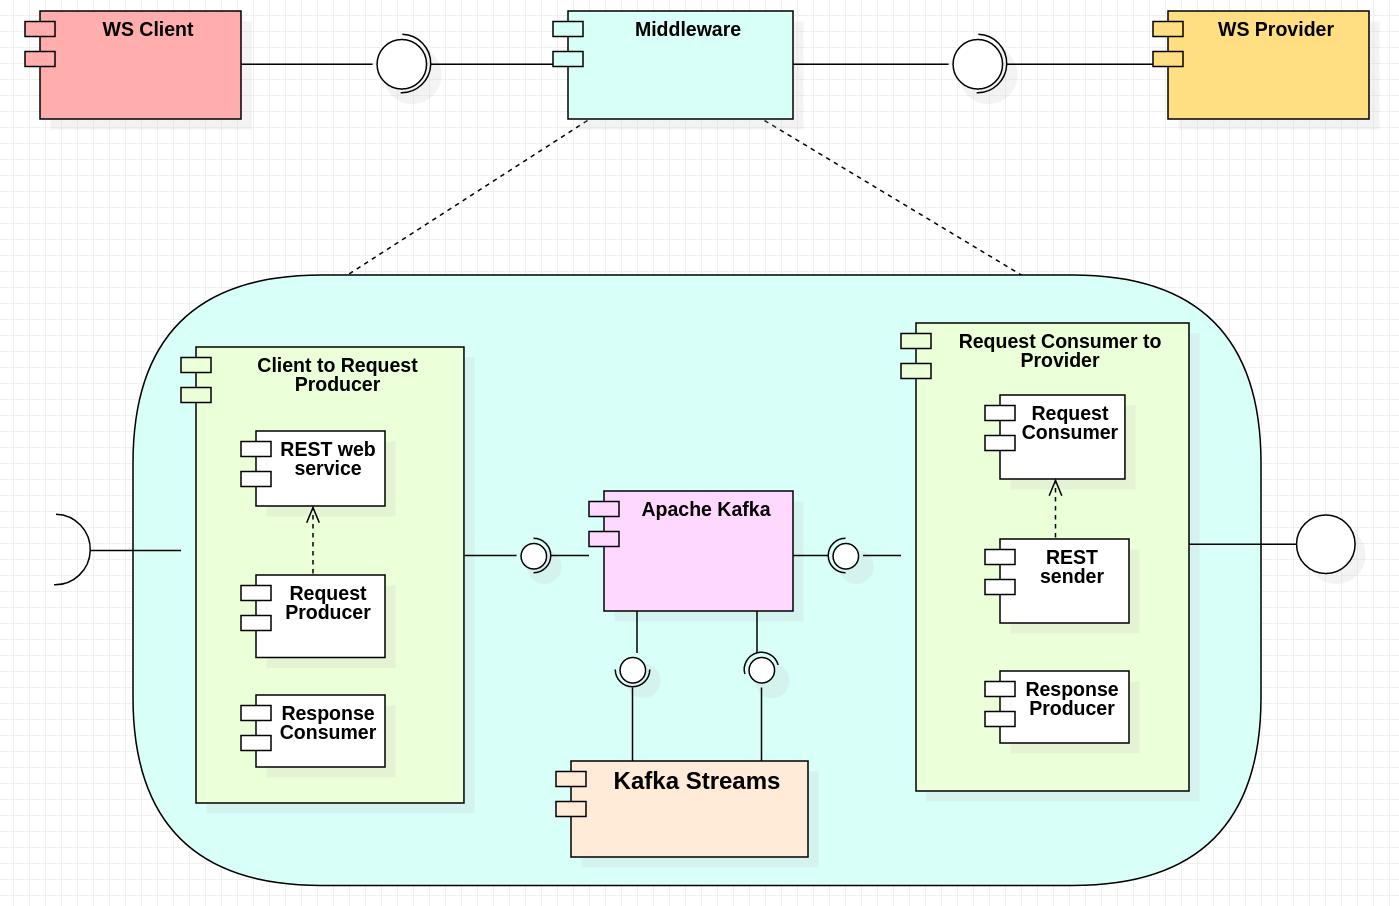
\includegraphics[width=\textwidth]{images/ap_component.png}
    \caption{\sacr{uml} \textit{component diagram} per la re-ingegnerizzazione del flusso asincrono (protetto)}
    \captionsetup{aboveskip=2pt}
    \caption*{\begin{footnotesize}\textit{Fonte: elaborazione personale}\end{footnotesize}}
  \end{center}
\end{figure}

Allo scopo di riassumere elegantemente i vari componenti del sistema ho elaborato un \sacr{uml} \textit{component diagram}.
Esso riassume con una visione ad alto livello i componenti che compongono il sistema e le modalità con cui esse interagiscono attraverso le relative interfacce.
% TODO: aggiungere testo


% , basati su delle immagini Linux leggere e personalizzate.

% Come si può vedere dalla figura \thefigure,

% \section{\textit{Setup} dell'ambiente di lavoro}


\section{Codifica}

\subsection{Kafka \textit{cluster}}

Il primo passo del processo di codifica è stato quello del \textit{setup} dell'ambiente di Kafka in locale.
La guida rapida online fornita direttamente da Apache per un'installazione minimale di Kafka porta al \textit{download} di un pacchetto e l'esecuzione di un servizio Zookeeper e un \textit{broker} di Kafka.

Zookeeper è un servizio attualmente essenziale al funzionamento di Kafka, gestisce i nodi del \textit{cluster} e mantiene una lista dei \textit{topic} e dei messaggi.
Le versioni future di Kafka renderanno questo servizio non necessario, ma attualmente sono ancora in fase di sviluppo e non adatta all'ambiente di produzione.
I due \textit{broker} si occupano di ricevere i messaggi dai \textit{producer}.

Dopo un breve collaudo del corretto funzionamento dei servizi tramite l'inserimento di un evento in un \textit{topic} e la relativa lettura, ho iniziato ad espandere e trasportare il sistema su dei \textit{container} Docker.

Il \textit{cluster} di Kafka utilizzato nel progetto di \stage\ è composto dai componenti descritti dalla progettazione architetturale nella sezione precedente, ovvero tre servizi di Zookeeper e due \textit{broker} per rappresentare un sistema di piccole dimensioni che tuttavia si avvicina ad un caso d'uso reale poiché contiene multipli Zookeeper e multipli \textit{broker}.

Questi cinque servizi necessitano dunque di eseguire contemporaneamente in un ambiente "containerizzato" con Docker connessi alla stessa \textit{network} locale, che consente ai diversi servizi di scambiare messaggi tra di essi.

Ho implementato questo \textit{cluster} tramite un
\textit{file} di tipo \texttt{yml} utilizzato dall'estensione Docker-compose.

\noindent
Il \textit{file} contiene una lista di servizi, in cui in ognuno viene specificato:
\begin{itemize}
  \item l'immagine Docker su cui viene costruito il servizio o il \texttt{dockerfile} da utilizzare per la sua costruzione;
  \item il nome del \textit{container};
  \item il nome del servizio;
  \item le dipendenze funzionali del servizio;
  \item l'indirizzo \sacr{ipv4} statico e le porte attraverso cui è possibile raggiungere il servizio all'interno della rete locale dagli altri \textit{container}.
\end{itemize}

\subsection{\textit{Request producer} e \textit{request conconsumer}}

Il passo successivo è stato quello di sviluppare dei semplici \textit{producer} e \textit{consumer} in grado di inserire e leggere i dati in Kafka.
Una volta collaudati rapidamente questi due eseguibili scritti in Java, li ho incapsulati all'interno di un'applicazione utilizzando lo strumento di \textit{build} e gestione delle dipendenze Maven\footfullcite{maven}.

Per completare il modulo che costituisce il prototipo di \middleware\ è necessario che il \textit{producer} e \textit{consumer} siano in grado di comunicare con dei servizi esterni e fornire le interfacce adatte al ruolo.
Nel caso più complesso del flusso asincrono con \textit{callback}, entrambi questi servizi devono essere in grado di restare in ascolto di eventuali \sacr{rest} \textit{request} (che nel mio progetto utilizzano il protocollo \sacr{http}) e al tempo stesso di inviarle.

Ho pertanto creato un \sacr{http} \textit{server} minimale in Java attraverso il \textit{framework} Netty\footfullcite{netty}, in esecuzione in un \textit{thread} Java.
Sviluppi futuri vedrebbero probabilmente l'utilizzo di un \textit{framework} più evoluto come Spring Boot\footfullcite{spring}.
Un altro \textit{thread} si occupa invece dell'invio delle \sacr{rest} \textit{request} al servizio di destinazione, una volta ricevuto un evento da parte del relativo \textit{consumer}.
Per abbreviare, chiamerò il servizio che si interpone tra il \sacr{ws} \textit{Client} e Kafka "\textit{request producer}", e quello che si interpone tra Kafka e \sacr{ws} \textit{Provider} "\textit{request consumer}", in base al loro scopo principale: essi inviano e ricevono la \textit{request} relativa al dialogo dal \textit{client} al \textit{provider}.
% \bigskip
\noindent
L'insieme di questi componenti formano i blocchi logici illustrati in verde nella sezione precedente, in cui il servizio \textit{request producer} è formato da:
\begin{itemize}
  \item \sacr{rest} \textit{\acrlong{ws}} (\sacr{http} \textit{server} in ascolto della \textit{client request});
  \item \textit{client request producer};
  \item \textit{callback request consumer};
  \item \sacr{rest} \textit{\acrlong{ws}} (invio della \textit{callback request});
\end{itemize}
\noindent
e il \textit{request consumer} da:
\begin{itemize}
  \item \textit{client request consumer};
  \item \sacr{rest} \textit{\acrlong{ws}} (invio della \textit{client request});
  \item \sacr{rest} \textit{\acrlong{ws}} (\sacr{http} \textit{server} in ascolto della \textit{callback request});
  \item \textit{callback request producer}.
\end{itemize}

\subsection{\sacr{ws} \textit{Client} e \sacr{ws} \textit{Provider} }

Al fine di testare il prototipo di \middleware\ prodotto, ho realizzato due ulteriori \textit{container} con all'interno due eseguibili che si occupano di interagire con esso.

Il servizio intitolato \sacr{ws} \textit{Provider} è fondamentalmente simile ai servizi descritti nella sotto-sezione precedente: anch'esso possiede un \sacr{http} \textit{server} per rimanere in ascolto delle \sacr{rest} \textit{request} inviate dal \textit{request consumer} oltre ad un metodo per elaborare la \sacr{rest} \textit{request} di risposta associata al \textit{callback}.

L'altro servizio, che idealmente potrebbe essere molto simile al precedente servizio di test, in realtà presenta delle considerevoli differenze.
La causa di ciò non è una differenza reale in termini di funzionalità, quanto una questione di rapidità di \textit{testing} e codifica.

Il servizio è molto più leggero in termini di memoria, essendo composto da un semplice \textit{container} con una distribuzione di Alpine Linux\footfullcite{alpine}; esso possiede un'installazione del \software\ \texttt{curl} (accessibile via \sacr{cli}), ma è privo di ulteriori \software\ aggiuntivi da me prodotti.

Gli obiettivi di questo \sacr{ws} \textit{Client} sono legati a due \textit{network utility}: \texttt{curl} e \texttt{netcat}.
La prima mi permette di eseguire, interagendo manualmente con il \textit{container} tramite l'interfaccia \sacr{cli}, di eseguire \sacr{rest} \textit{request} con il \sacr{json} di partenza.
La seconda mi consente di restare in ascolto di eventuali \textit{request} su di una porta a mia scelta.

% I vantaggi di questa modalità manuale risiedono come anticipato nello sviluppo rapido, non solo di questo servizio ma anche dei restanti.
% Infatti grazie alle funzioni offerte da docker-compose, è semplice eseguire il \textit{restart} di un singolo \textit{container} contenente un servizio per testarne la nuova versione, e successivamente è sufficiente eseguire manualmente la \textit{request} dal \sacr{ws} \textit{Client} per verificare il funzionamento del sistema.

\subsection{Protezione dei dati sensibili con Kafka Streams}

Come visto nella sezione \ref{sec:progettazione}, alcuni dei dati trasmessi nel \sacr{json} vengono trasformati per mascherare i dati sensibili.

\noindent
Precisamente, il \sacr{json} passa dall'avere questa forma
% {\sacr{json} inviato al \middleware}
\begin{figure}[H]
  \begin{mycode}{json}
    {
      "CallerSystem": "Sistema chiamante 1",
      "PhoneNumber": "012345679",
      "Currency": "EUR",
      "Amount": "5",
      "Info": "Causale del Trasferimento Credito Residuo",
      "DebitType":"Bancomat",
      "CreditTransferDate": "2021-07-21",
      "CreditCardNumber": "1234567890123456"
    }
  \end{mycode}
  \caption{{\sacr{json} inviato al \middleware}}
  \captionsetup{aboveskip=2pt}
  \caption*{\begin{footnotesize}\textit{Fonte: elaborazione personale}\end{footnotesize}}

\end{figure}
\noindent
a questa
\begin{figure}[H]
  \begin{mycode}{json}
    {
      "CallerSystem": "Sistema chiamante 1",
      "PhoneNumber": "012345679",
      "Currency": "EUR",
      "Amount": "5",
      "Info": "Causale del Trasferimento Credito Residuo",
      "DebitType":"Bancomat",
      "CreditTransferDate": "2021-07-21",
      "CreditCardNumber": "****************"
    }
  \end{mycode}
  \caption{\sacr{json} protetto, ricevuto al termine del \textit{callback}}
  \captionsetup{aboveskip=2pt}
  \caption*{\begin{footnotesize}\textit{Fonte: elaborazione personale}\end{footnotesize}}
\end{figure}
\noindent
in cui si può notare che l'ultimo dato ha subito la modifica descritta.

Ho implementato questa funzione utilizzando Kafka Streams\footfullcite{streams}, che permette di leggere un \textit{topic} e modificarlo istantaneamente per un'elaborazione in \textit{real time}.

\subsection{Efficienza nello sviluppo}

Durante la codifica, ho adottato diverse misure per minimizzare il tempo necessario.
Questi provvedimenti riguardano principalmente l'ottimizzazione del sistema di \textit{container}, non allo scopo di migliorare l'efficienza, rapidità d'esecuzione e di \textit{build} del prodotto finale (che è stata comunque raggiunta come effetto secondario) ma a quello di ridurre il tempo e risorse necessarie per il \textit{testing}, riducendo di conseguenza le ore e le risorse necessarie allo sviluppo.

Tutti le misure prese sono strettamente legate alla mia famigliarità con alcune tecnologie e al risorse personali richieste per l'apprendimento e sviluppo di una nuova funzionalità.

\noindent
Elenco i principali provvedimenti intrapresi per minimizzare il tempo di sviluppo:
\begin{itemize}
  \item \textbf{ottimizzazione delle risorse utilizzati dai \textit{container}}.
  Molti dei container prodotti possiedono delle versioni \textit{premade} sulla libreria di DockerHub\footfullcite{dockerhub} (ad esempio i \textit{container} che formano il \textit{cluster} di Kafka).
  Tuttavia, utilizzare delle versioni \textit{ad-hoc} da me costruite mi ha permesso di ridurre considerevolmente le dimensioni del \textit{container} e mantenere solamente le funzioni a me necessarie, e conseguentemente ridurre il tempo della \textit{build} delle immagini e la loro esecuzione. Dato le numerose operazioni di \textit{build} e \textit{testing}, nel lungo termine ha portato ad un risparmio di tempo significativo.
  \item \textbf{invio della richiesta \sacr{rest} del \textit{service client} tramite \sacr{cli}}.
  I vantaggi di questa modalità manuale risiedono come anticipato nella rapidità di sviluppo, non solo di questo servizio ma anche dei restanti.
  Infatti grazie alle funzioni offerte da docker-compose, è semplice eseguire il \textit{restart} di un singolo \textit{container} contenente un servizio per testarne la nuova versione, e successivamente è sufficiente eseguire manualmente la \textit{request} dal \sacr{ws} \textit{Client} per verificare il funzionamento del sistema.
  È sicuramente possibile l'automatizzazione di questo processo (ad esempio effettuando richieste continue in modo automatico) ma l'implementazione di questa funzione avrebbe, secondo la mia stima personale, richiesto più tempo della soluzione attuata o posto problemi nel filtro dell'\textit{output}.
  \item \textbf{la \textit{build} delle applicazioni costruite con Maven avviene in locale}.
  Questo porta a due vantaggi.
  Il primo è che la \textit{build} impiega meno tempo, dato che non è necessario lanciare alcun \textit{container} e Maven non deve sincronizzare o controllare la versione delle dipendenze online più di volte (è possibile  disattivare la sincronizzazione, ma richiede comunque più tempo).
  La seconda, più importante, è che l'immagine Docker stessa non richiede né \textit{build} né Maven.
  Il \textit{container} si occupa solamente di copiare l'eseguibile pre-costruito al suo interno e di eseguirlo con Java.
\end{itemize}

\section{Prodotto finale, verifica e collaudo}

Il prodotto finale del progetto è composto da i diversi componenti illustrati nella sotto-sezione \ref{sub:uml_component}, per un totale di dieci servizi ognuno nel proprio
\textit{container} Docker (conformi con il \textit{deployment diagram} alla sotto-sezione \ref{sub:uml_deployment}).
Tre di questi servizi risultano più strutturati e complessi, ovvero il \textit{request producer}, \textit{request consumer} e il \sacr{ws} \textit{Provider}.
Questi infatti sono degli applicativi \textit{multi-thread}, con struttura generata da Maven e formati da diversi \texttt{file} Java che si occupano di inviare e ricevere \sacr{rest} \textit{request}, "produrre" e "consumare" i dati utilizzando Kafka.

\begin{figure}[H]
  \begin{center}
    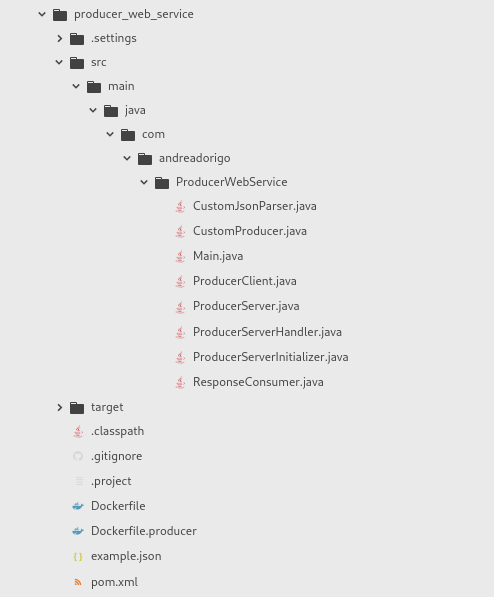
\includegraphics[width=0.5\textwidth]{images/folder_tree.png}
    \caption{\textit{Folder tree} dell'applicativo relativo al servizio \textit{request producer}}
    \caption*{\begin{footnotesize}\textit{Fonte: elaborazione personale}\end{footnotesize}}
  \end{center}
\end{figure}

I cinque servizi del \textit{cluster} di Apache Kafka risultano relativamente semplici: sono composti da un'immagine di Alpine Linux con un'installazione di Java \sacrfoot{jre} versione 8, con all'interno gli eseguibili di Kafka e i file di configurazione personalizzati.

% TODO: completare con i 2 servizi rimanenti


Nella figura \ref{fig:riass_componenti} è presente una bozza riassuntiva dalla \textit{board} di progetto ClickUp.

\begin{figure}[h]
  \begin{center}
    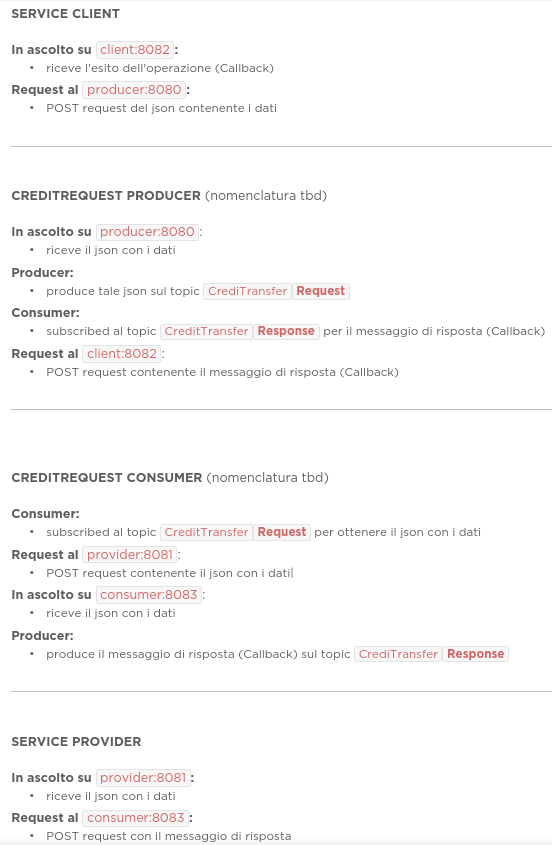
\includegraphics[width=0.63\textwidth]{images/riass_componenti.png}
    \caption{\sacr{uml} Riassunto dei componenti prodotti nel caso asincrono con \textit{callback} e della loro comunicazione}
    \captionsetup{aboveskip=2pt}
    \caption*{\begin{footnotesize}\textit{Fonte: elaborazione personale}\end{footnotesize}}
    \label{fig:riass_componenti}
  \end{center}
\end{figure}

L'immagine illustra i servizi prodotti per il flusso asincrono con \textit{callback} e di come essi comunichino tra di loro attraverso le varie porte, elaborata durante il processo di Progettazione iniziale (in cui non è ancora presente la protezione del dato sensibile con Kafka Streams).

Una visione ad alto livello può esprimere il prodotto risultante dallo \stage\ come \textbf{due servizi di test quali \sacr{ws} \textit{Client} e \sacr{ws} \textit{Provider} che scambiano messaggi sotto forma di \texttt{file} \sacr{json} tramite un \middleware\ basato su Apache Kafka in un'architettura focalizzata sugli eventi.}
Il\middleware\ presenta inoltre la funzionalità aggiuntiva di trasformazione dei dati grazie all'utilizzo di Kafka Streams.
% Questi microservizi hanno raggiunto efficacemente il risultato preposto, creando il sistema richiesto dalla sperimentazione; i due servizi di test quali \sacr{ws} \textit{Client} e \sacr{ws} \textit{Provider} si scambiano messaggi tramite un \middleware\ basato su Apache Kafka.

A seguito di tutte le dovute verifiche del \software, il prodotto è stato più volte collaudato con la supervisione del tutor aziendale e il responsabile del \sacr{eai}.
Tutti i \textit{container} prodotti sono stati revisionati, compresa la loro corretta esecuzione.

Il tempo dedicato al processo di Collaudo è stato relativamente breve rispetto alla maggior parte dei prodotti \software: la causa di questa durata minore è la natura sperimentale del progetto di \stage\ che, come visto nella sotto-sezione \ref{sub:obiettivi_stage}, è incentrato sulla re-ingegnerizzazione del flusso di dati ma senza l'obiettivo di produrre un \middleware\ da implementare in produzione (quest'ultimo è un obiettivo aziendale nel lungo termine, ma non di questo specifico progetto di sperimentazione).

Questi collaudi hanno visto il processo di \textit{build} e successivo avvio simultaneo di ogni singolo servizio all'interno del \textit{cluster} tramite l'apposito comando di Docker-compose "\texttt{docker-compose up --build}".
Dopodiché, al fine di testare che il \software\ eseguisse effettivamente le funzioni richieste dal progetto di sperimentazione (\textit{test} d'efficacia), ho effettuato delle \sacr{http} \sacr{rest} \textit{request} contenenti il \sacr{json} con i dati.
Ho eseguito questo processo connettendomi al \textit{container} contenente il servizio \sacr{ws} \textit{client}, per poi dare manualmente il comando di \textit{request} grazie all'\textit{utility} \texttt{curl}.
L'analisi del \sacr{json} in entrata e in uscita da ogni servizio mi ha garantito l'efficacia del \software\ sperimentale prodotto.

Infine, il prodotto finale è stato presentato all'azienda in conclusione del percorso di \stage\ in un \textit{online meeting} con l'aiuto di alcune diapositive da me prodotte e una dimostrazione \textit{live} del \software\ in esecuzione tramite la condivisione dello schermo.

% Come si può osservare

\chapter{Valutazione retrospettiva}

% \section{Obiettivi soddisfatti dallo stage}
%
% Valutazione oggettiva riguardo il percorso e i risultati raggiunti da esso.
%
% \section{Maturazione professionale acquisita}
%
% Descrizione delle conoscenze e abilità professionali acquisite grazie al percorso di \textit{stage}.
% Valutazione del miglioramento personale portato avanti durante il percorso di stage.
%
%
% \section{Distanza tra le competenze necessarie e quelle acquisite nel corso di studi}
%
% Breve valutazione riguardo le difficoltà riscontrate, e considerazioni riguardo le competenze ottenute durante il corso di laurea che più mi hanno aiutato durante il percorso.
\section{Obiettivi aziendali raggiunti}

L'azienda ha potuto testare, con questo percorso di \stage, le potenzialità di Apache Kafka nell'ambito dei \middleware\ e dei sistemi di integrazione.
La piattaforma di \textit{event streaming} risulta molto promettente da integrare negli attuali e futuri sistemi di integrazione basati su di un \acrlong{eda}, al fine di soddisfare i bisogni del cliente della gestione di un flusso di dati sempre maggiore, in tempo reale.
Il \software\ può portare dunque a una grande innovazione nel settore \sacr{eai} e permettere a Sync Lab di fornire prodotti all'avanguardia ai suoi clienti.

Inoltre, durante questi mesi di \stage, l'azienda ha avuto modo di conoscere il mio metodo di lavoro e le mie capacità.

Il tutor aziendale e gli esperti del settore mi hanno fornito un riscontro molto positivo, sia riguardo i risultati raggiunti dallo \stage\ che riguardo le mie capacità e maturazione professionale osservate durante il percorso.

\section{Obiettivi dello stage raggiunti}

Gli obiettivi principali dello stage sono stati raggiunti con successo.

I \gls{g_microservizi} che compongono il prodotto finale hanno raggiunto efficacemente il risultato inizialmente previsto, creando il sistema richiesto dalla sperimentazione; i due servizi di test quali \sacr{ws} \textit{Client} e \sacr{ws} \textit{Provider} si scambiano messaggi tramite un \middleware\ basato su Apache Kafka.

La sperimentazione ha testato alcune delle capacità di Apache Kafka con esito positivo, fornendo le basi per ulteriori percorsi di approfondimento che possono portare all'implementazione della piattaforma di \textit{event streaming} all'interno degli attuali sistemi di integrazione con il ruolo di \middleware.

Un possibile percorso potrebbe ad esempio modellare e sviluppare un caso d'uso molto più complesso, con simulazione di un flusso di dati continuo e di grandi dimensioni, con dati provenienti da fonti multiple, un numero maggiore di \textit{producer} e \textit{consumer}, e la sperimentazione di ulteriori funzionalità presenti nei \middleware\ attualmente utilizzati.

\noindent
Di seguito viene ripresa parte della tabella \ref{tab:pianificazione} vista nella sezione \ref{sec:pianificazione}.

\onehalfspacing
\begin{small}
  \begin{center}
    \centering
    \renewcommand\arraystretch{1.6}
    \begin{longtable}{| >{\centering\arraybackslash}m{2cm}|m{9.5cm}|>{\centering\arraybackslash}m{2.2cm}|}
      \hline
      \textsc{\textbf{Obiettivo}} & \textsc{\textbf{Task associati}} & \textsc{\textbf{Raggiunto}} \\
      \hline
      O-5.1 & Analisi dei casi d'uso reali & \textsc{si} \\
      \hline
      O-5.2 & Realizzazione dei componenti per l'esecuzione dei casi di test & \textsc{si}\\
      \Xhline{2\arrayrulewidth}
      O-6.1 & Analisi re-ingegnerizzazione e collaudo del flusso di integrazione asincrono & \textsc{si} \\
      \Xhline{2\arrayrulewidth}
      O-7.1 & Analisi e re-ingegnerizzazione e collaudo del flusso di integrazione asincrono con callback & \textsc{si}\\
      \Xhline{2\arrayrulewidth}
      O-8.1 & Analisi e re-ingegnerizzazione e collaudo del flusso di integrazione sincrono & \textsc{no}\\
      \hline
      % \textsc{Non previsto} & Sperimentazione di funzioni aggiuntive: protezione di un dato sensibile & \textsc{si}\\
      % \hline

      \caption{Obiettivi dello stage raggiunti}
    \end{longtable}
  \end{center}
\end{small}
% \doublespacing

Come detto in precedenza, l'obiettivo O-8.1 è stato scartato in favore della sperimentazione di alcune funzioni aggiuntive di Kafka, inizialmente non pianificate.

% \section{Prodotti sviluppati}
%
% Il prodotto finale del progetto è composto da i diversi componenti illustrati nella sottosezione \ref{sub:uml_component}, per un totale di dieci servizi ognuno nel proprio
% \gls{g_container} Docker (conformi con il \textit{deployment diagram} alla sottosezione \ref{sub:uml_deployment}).
%
% Questi \gls{g_microservizi} hanno raggiunto efficacemente il risultato preposto, creando il sistema richiesto dalla sperimentazione; i due servizi di test quali \sacr{ws} \textit{Client} e \sacr{ws} \textit{Provider} si scambiano messaggi tramite un \middleware\ basato su Apache Kafka.

\section{Contenuti formativi acquisiti}

Il processo di Formazione ha riguardato principalmente i concetti inerenti al settore del \textit{\acrlong{eai}} e le tecnologie legate ad Apache Kafka.

Di seguito espongo i requisiti formativi soddisfatti, in relazione al piano di lavoro iniziale.

\onehalfspacing
\begin{small}
  \begin{center}
    \centering
    \renewcommand\arraystretch{1.6}
    \begin{longtable}{| >{\centering\arraybackslash}m{2cm}|m{9.5cm}|>{\centering\arraybackslash}m{2.2cm}|}
      \hline
      \textsc{\textbf{Obiettivo}} & \textsc{\textbf{Task associati}} & \textsc{\textbf{Raggiunto}} \\
      \hline
     %  O-1.1 & Incontro con le persone coinvolte nel progetto per discutere i requisiti e le richieste relative al sistema da sviluppare & \textsc{si} \\
     %  \hline
     %  O-1.2 & Verifica credenziali e strumenti di lavoro assegnati & \textsc{si}\\
     %  \hline
     %  O-1.3 & Presa visione dell’infrastruttura esistente & \textsc{si}\\
     %  \hline
     %  D-1.1 & Ripasso approfondito riguardo i seguenti argomenti:
     %    \smallskip
     %    \begin{itemize}
     %       \item Ingegneria del \software;
     %       \item Sistemi di versionamento;
     %       \item Architetture \software;
     %       \item Cenni di \textit{Networking}.
     %     \end{itemize} &  \textsc{si}\\
     % \Xhline{2\arrayrulewidth}
     O-2.1 & Nozioni fondamentali riguardo \sacr{eai} e \sacr{soa} & \textsc{si}\\
     \hline
     O-2.2 & Approfondimenti riguardo le Architetture a Messaggio
       % \begin{itemize}
       %    \item \textit{Integration Styles};
       %    \item \textit{Channel Patterns};
       %    \item \textit{Message Construction Patterns};
       %    \item \textit{Routing Patterns};
       %    \item \textit{Transformation Patterns};
       %    \item \textit{System Management Patterns}.
       %  \end{itemize}
         & \textsc{si}\\
    \Xhline{2\arrayrulewidth}

    O-3.1 & Apache Kafka
      % \begin{itemize}
      %     \item Introduzione a Kafka;
      %     \item Concetti fondamentali di Kafka;
      %     \item Avvio e \sacr{cli};
      %     \item Programmazione in Kafka con Java.
      %   \end{itemize}
        & \textsc{si}\\
    \hline
    D-3.1 & Esempi e applicazioni di Apache Kafka & \textsc{si} \\
    \Xhline{2\arrayrulewidth}

    O-4.1 & Confluent Platform
      % \begin{itemize}
      %     \item \textit{Service registry};
      %     \item \sacr{rest} \textit{proxy};
      %     \item kSQL;
      %     \item Confluent \textit{connectors};
      %     \item \textit{Control center}.
      % \end{itemize}
       & \textsc{si}\\
    \Xhline{2\arrayrulewidth}


      \caption{Contenuti formativi acquisiti}
    \end{longtable}
  \end{center}
\end{small}
% \doublespacing

\section{Obiettivi personali raggiunti}
%
% - molto soddisfacenti
%
% - espansione delle conoscenze tecnologiche
%
% - maturazione professionale
%
% - inserimento in un contesto Aziendale
%
% - gestione e organizzazione di progetto
Valuto i risultati personali raggiunti dal percorso di \stage\ molto soddisfacenti, soprattutto dal punto di vista di una maturazione professionale.

La formazione ricevuta nel settore del \textit{\acrlong{eai}} ha allargato le mie conoscenze tecnologiche nell'ambito dell'ingegneria del \software; in particolare ho apprezzato l'approfondimento riguardo le architecture \software\ moderne e i sistemi di integrazione associati al mondo del \textit{Big Data}.
Ho apprezzato molto lo studio delle tecnologie emergenti per un'innovazione aziendale nel \sacr{eai}, quali Apache Kafka e Confluent, e le conseguenze importanti dovute alla migrazione di un sistema verso una \acrlong{eda}.

L'alto livello di organizzazione personale che ho tenuto durante il percorso ha garantito un buona qualità nel \textit{way of working}, preparandomi all'inserimento nel mondo del lavoro e a un contesto aziendale innovativo e all'avanguardia.

Gli esperti aziendali che mi hanno fornito il supporto e le linee guida necessarie al compimento dello \stage\ sono stati per me una grande fonte di apprendimento; in particolare, ho imparato gli importanti passi e considerazioni necessarie che guidano la sperimentazione associata all'implementazione di tecnologie innovative, sia in ambito tecnico che architetturale.

\begin{figure}[h]
  \begin{center}
    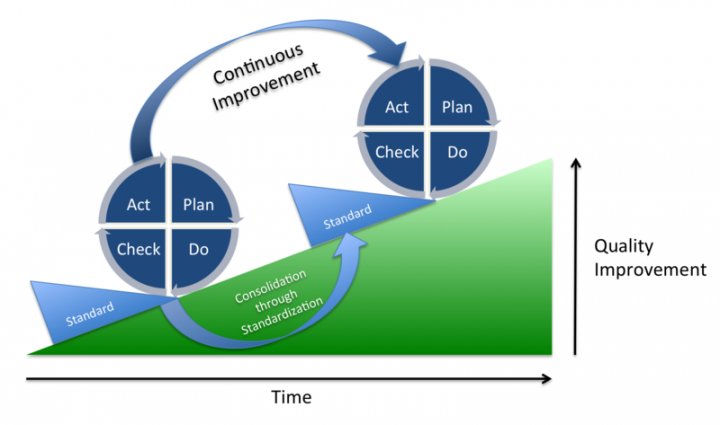
\includegraphics[width=0.85\textwidth]{images/pdca.png}
    \caption{\acrlong{pdca}}
    \captionsetup{aboveskip=2pt}
    \caption*{\begin{footnotesize}\textit{Fonte:} \url{http://quickstart-indonesia.com/siklus-pdca/}\end{footnotesize}}
  \end{center}
\end{figure}

L'adozione del \sacrfoot{pdca} (figura \thefigure) nel mio metodo di lavoro è stato essenziale per dei miglioramenti personali in diversi ambiti, soprattutto quelli legati alla gestione del tempo (come visto nella sotto-sezione \ref{subsub:auto-miglioramento}), efficienza organizzativa ed efficacia di sviluppo.

Ritengo dunque di aver raggiunto tutti gli obiettivi personali posti, con risultati addirittura migliori delle mie aspettative iniziali.

\section{Distanza rispetto ai contenuti del corso di studi}

Nonostante le tecnologie e i concetti utilizzati nel percorso siano stati per me una novità rispetto agli insegnamenti previsti nel Corso di Laurea, \textbf{ritengo che il percorso di studi abbia completamente soddisfatto i requisiti necessari per il completamento dello \stage.}

Infatti, sebbene gli insegnamenti non abbiano specificatamente trattato le moderne tecnologie utilizzate, mi hanno fornito la preparazione necessaria al loro  rapido apprendimento; in un settore lavorativo in rapida evoluzione come quello dell'informatica, la capacità di adattamento all'utilizzo di strumenti moderni come Apache Kafka e quella di comprendere facilmente le architetture innovative è di fondamentale importanza e personalmente molto apprezzata.

% Alcuni corsi in particolare hanno provveduto sostanzialmente la distanza tra l'ambiente universitario e quello lavorativo, quali ingegneria del software (con progetto associato), basi di dati, tecnologie web, e i vari corsi di programmazione.
Mi ritengo pertanto pienamente soddisfatto del percorso di studi e soprattutto del percorso di \stage; ritengo essi abbiano dato una rapida accelerazione alla mia formazione professionale e abbia fornito i presupposti necessari per un mio inserimento nell'ambiente lavorativo.


% TODO: In §4.4 non menzionerai specifici insegnamenti, neanche in positivo, ma ragionerai sul complesso del percorso di studi.


\printglossary[type=\acronymtype]
\printglossary

\printbibliography
% \clearpage{\pagestyle{plain}\cleardoublepage} %Numerazione araba per i capitoli
% \pagenumbering{arabic}
%
%
% \clearpage{\pagestyle{plain}\cleardoublepage} %Comando per iniziare il capitolo su pagina dispari
% \chapter{Primo Capitolo} %Nome capitolo
% \label{chapter:primo_capitolo} %Label per creare riferimenti al capitolo
% \input{intro_cap1.tex} %File in cui verrà scritto il capitolo
%
% \clearpage{\pagestyle{plain}\cleardoublepage}
% \chapter{Immagini e Tabelle}
% \label{chapter:immagini_e_tabelle}
% \input{intro_cap2.tex}
%
% \clearpage{\pagestyle{plain}\cleardoublepage}
% \chapter{Formule}
% \label{chapter:formule}
% \input{intro_cap3.tex}
%
% \clearpage{\pagestyle{plain}\cleardoublepage}
% \chapter{Pseudocodice e codice}
% \label{chapter:codice}
% \input{intro_cap4.tex}
%
% \clearpage{\pagestyle{plain}\cleardoublepage}
% \input{bibliografia.tex}

\end{document}
